\chapter{Background}\label{chap:background}

The following part is to provide a short introduction into the theory of reinforcement learning, the Soft Actor Critic Algorithm (SAC) as well to Variational Autoencoders (VAE) and Conditional Variational Autoencoders (CVAE). In the end we will explain the concepts behind forward and inverse kinematics and go deeper into the algorithm representing a expert for inverse kinematics, Cyclic Coordinate Descent (CCD).

The following sections are a summary of the present work from several different groups and researchers. For more details please refer to their original publications or to more sophisticated literature like the textbook ``Reinforcement Learning: An Introduction'' from Richard Sutton and Andrew Barto~\cite{SuttonBartoRLBook}, ``Deep Learning'' from Ian Goodfellow, Yoshua Bengio and Aaron Courville~\cite{DeepLearningTextBook} and ``Probabilistic Machine Learning: Advanced Topics'' from Kevin Murphy~\cite{pml2Book}. 

\section{RL Framework}\label{sec:RL-Framework}

Learning is a topic that is present in all our lives since their beginning. We all learn to move our arms, like an infant that is wiggling around, learn to walk, to speak and more or less any other skill that we find in our personal repository until now.  

Reinforcement Learning (RL) is a computational approach based on learning by doing, where an agent interacts with an environment to maximize a reward. RL problems, like riding a bicycle, present challenges without explicit instructions for achieving the goal. They involve a closed-loop system where actions yield feedback, whether immediate (e.g., not crashing a bike) or delayed (e.g., earning a bonus in a board game). RL problems can be characterized by three key features:

\begin{itemize}
    \item Closed-loop interaction between actions and environment feedback.
    \item Lack of explicit problem-solving instructions for the agent.
    \item Actions having consequences over time for the agent or the environment.
\end{itemize}

Before we can have an exemplary look on the closed loop mechanics, we would like to introduce a couple of key components of RL including the Markov Decision Process.

% \begin{figure}
	\centering
	\minipage{0.5\textwidth}
    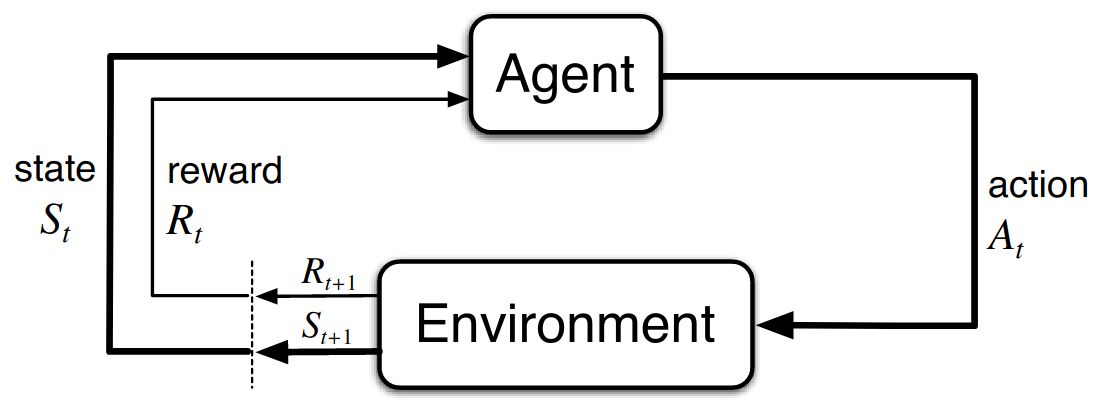
\includegraphics[width=\linewidth,]{figures/background/agent-environment-interaction.png}
	\caption{interaction between agent and the environment}
	\label{fig:agent-environment_interaction}
	\endminipage
\end{figure}



\begin{figure}
	\centering
	\minipage{0.7\textwidth}
    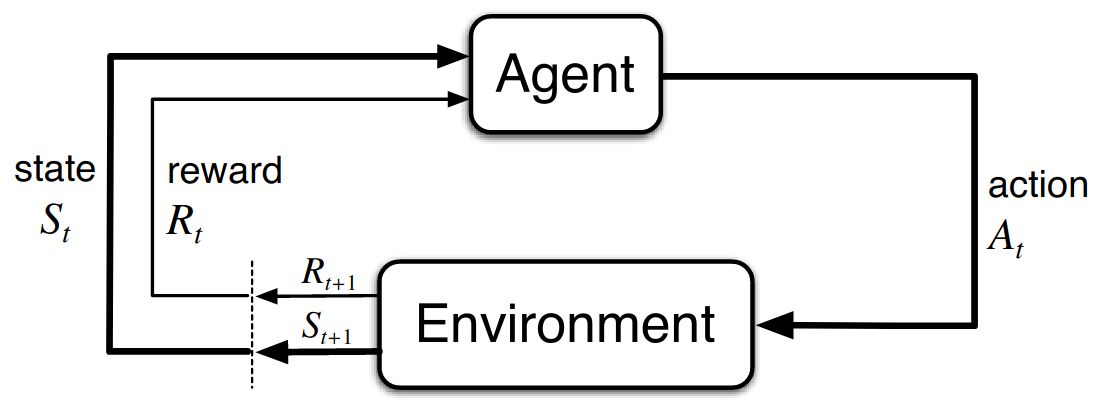
\includegraphics[width=\linewidth,]{figures/background/agent-environment-interaction.png}
	\caption[Interaction between agent and environment]{interaction between agent and the environment is living in to pursue his goal. Figure is kindly provided by R. Sutton and A. Barto in ``Reinforcement Learning: An Introduction''~\cite{SuttonBartoRLBook}}
	\label{fig:agent-environment_interaction}
	\endminipage
\end{figure}

Every agent exists in a specified environment and also interacts within a sequence of discrete time steps $t \in \mathbb{N}$. In order to do so the agent has to perceive the environment through a \textbf{state} representation $S_t \in \mathcal{S}$ which is an element of all possible states, the state space $\mathcal{S}$. To interact with the environment the agent has to perform an \textbf{action} $A_t \in \mathcal{A}(S_t)$ where $\mathcal{A}(S_t)$ is the set of all possible actions in given state $S_t$. To chose an action the agent calculates for each possible action $A_t$ a probability $\pi_{\theta, t}(A_t|S_t)$ for a given state $S_t$ and samples from an action from this distribution. To achieve a more compact notation we will refer to the action $A_t = a$ and the state $S_t = s$. Further we refer to the policy always as a parameterized policy $\pi_\theta = \pi_{\theta, t}(a|s)$.  
This probability distribution is called the \textbf{policy}. 
After the agent has chosen and executed an action, which also means the environment will move one time step further $t \to t + 1$, the environment will return the next state $S_{t+1}$ and the agent will perceive a \textbf{reward} $R_{t+1} \in \mathbb{R}$ with $\mathbb{R}$ as the set of all possible rewards.\\
The long term goal of the agent is to adapt its policy to maximize the total amount reward the agent receives from the environment.
These key terminology can also be found in the notation of a Markov Decision Process which is classified as a 4-Tuple of: $(\mathcal{S}, \mathcal{A}, P_a(s, s'), R_a(s, s'))$ with $ P_a(s, s')$ as a probability distribution that action $a$ in state state $s$ will lead to the next state $s' = s_{t+1}$ and $ R_a(s, s')$ as reward function for transitioning from $s$ to $s'$ with $a$~\cite{SuttonBartoRLBook}.

The overall goal of an agent is to maximize its received cumulative return $G_t$ for one run until time step $T$~\cite{SuttonBartoRLBook}. This is metric is denoted in~\eqref{eqn:discounted-cumulative-return}. In~\eqref{eqn:discounted-cumulative-return} $\gamma$ is the discount rate, $0 \leq \gamma \leq 1$, a parameter to regularize the \textit{importance} of individual received rewards over time. 

\begin{align}
	G_t & \ \dot{=} \sum_{k=t+1}^T \gamma^{k-t-1}R_k \label{eqn:discounted-cumulative-return} \\
	&= R_{t+1} + \gamma G_{t+1} \label{eqn:discounted-cumulative-return-recursive}
\end{align}

Due to the dependence of individual rewards $R_t$ on state-action pairs from the same time step $t$, we can not compute the received cumulative return until the episodes end. To solve this problem reinforcement learning algorithms try to maximize the expected return $v_{\pi_\theta}(s)$ as in~\eqref{eqn:expected-return}~\cite{SuttonBartoRLBook}, or value function, for a given state. For Markov decision process we can define the value function as in~\eqref{eqn:Bellman-valuefunction}~\cite{SuttonBartoRLBook}. 

\begin{align}
	% v_{\pi_\theta}(s) = \sum_a \pi_\theta(a|s) \sum_{s', r} P(s', r| s, a)\left[r + \gamma v_{\pi_\theta}(s'm)\right] 
	v_{\pi_\theta}(s) & \ \dot{=} \ \mathbb{E}_{\pi_\theta}[G_t | S_t = s] \label{eqn:expected-return} \\
	&\overset{\mathclap{\strut(\ref{eqn:discounted-cumulative-return-recursive})}}{=} \mathbb{E}_{\pi_\theta}[R_{t+1} + \gamma G_{t+1}| S_t = s] \nonumber \\
	& = \sum_a \pi_\theta(a|s) \sum_{s'} \sum_r P(s', r| s, a)\left[r + \gamma \mathbb{E}_{\pi_\theta}[G_{t+1} | S_{t+1} = s']\right] \nonumber \\
	& = \sum_a \pi_\theta(a|s) \sum_{s', r} P(s', r| s, a)\left[r + \gamma v_{\pi_\theta}(s'm)\right] \label{eqn:Bellman-valuefunction}
\end{align}

For a finite Markov decision process we can also define a the optimal value function $v_*(s)$ with respect to the optimal policy in~\eqref{eqn:Bellman-optimal-valuefunction} adapted from Sutton and Barto~\cite{SuttonBartoRLBook}.

\begin{equation}\label{eqn:Bellman-action-valuefunction}
	q_{\pi_\theta}(s, a) = \sum_{s', r} P(s', r |s, a) \left[r + \gamma \sum_{a'} \pi_\theta(a'| s')q_{\pi_\theta}(s', a')\right]
\end{equation}

\begin{align}
	v_*(s) & \ \dot{=} \max_{\pi_\theta} v_{\pi_\theta}(s) \label{eqn:optimal-valuefunction} \\
	&=\max_a \sum_{s', r} P(s', r| s, a)[r + \gamma v_*(s')] \label{eqn:Bellman-optimal-valuefunction}
\end{align}

Because~\eqref{eqn:optimal-valuefunction} holds we can formulatethe reinforcement learning problem as in~\eqref{eqn:RL-policy-problem} for the optimal policy $\pi_\theta^*$ and with respect to a performance measure $J(\pi_\theta) = \mathbb{E}_{\pi_\theta}[G_t | S_t = s]$ as:
\begin{align}
	\pi_\theta^* &= \arg \max_{\pi_\theta}J(\pi_\theta) \label{eqn:RL-policy-problem} \\
	&= \arg \max_{\pi_\theta} \mathbb{E}_{\pi_\theta}[G_t | S_t = s] \\
	&\overset{\mathclap{\strut(\ref{eqn:expected-return})}}{=} \arg \max_{\pi_\theta} v_{\pi_\theta}(s) \label{eqn:RL-policy-valuefunction}
\end{align}

\begin{equation}\label{eqn:Bellman-optimal-action-valuefunction}
	q_*(s, a) = \sum_{s', r} P(s', r|s, a)\left[r + \gamma \max_{a'} q_*(s', a')\right]
\end{equation}

\section{Generalized Policy Iteration}\label{sec:Generalized-Policy-Iteration}

This section is about to provide an introduction to the idea of policy iteration. For a more detailed look into the topic it is recommended refer to the Reinforcement Learning Textbook from Richard Sutton and Andrew Barto~\cite{SuttonBartoRLBook}.

One fundamental concept for reinforcement learning algorithms is policy iteration. At Its core it is described as the alternating interaction between a policy improvement step and a policy evaluation step as in \figref{fig:policy-iteration-concept}. This interaction goes back and forth during the execution of most reinforcement learning algorithms until a state of convergence in the value function and policy has arrived. That means both value function and policy are optimal for the given problem. This state can be reached if the ``value function is consistent with the current policy, and the policy stabilizes only when it is greedy with respect to the current value function''. This can be also seen in the Bellman optimally equation as in~\eqref{eqn:Bellman-optimal-valuefunction}. 

% \begin{figure}
    \begin{center}
        
\includegraphics[width=0.5\linewidth]{figures/place_holder.png}
        \caption[policy iteration concept]{\textbf{schematic drawing of a conditional Variational Autoencoder}}
        \label{fig:policy-iteration-concept}
    \end{center}
\end{figure}
\begin{figure}
    \begin{center}
        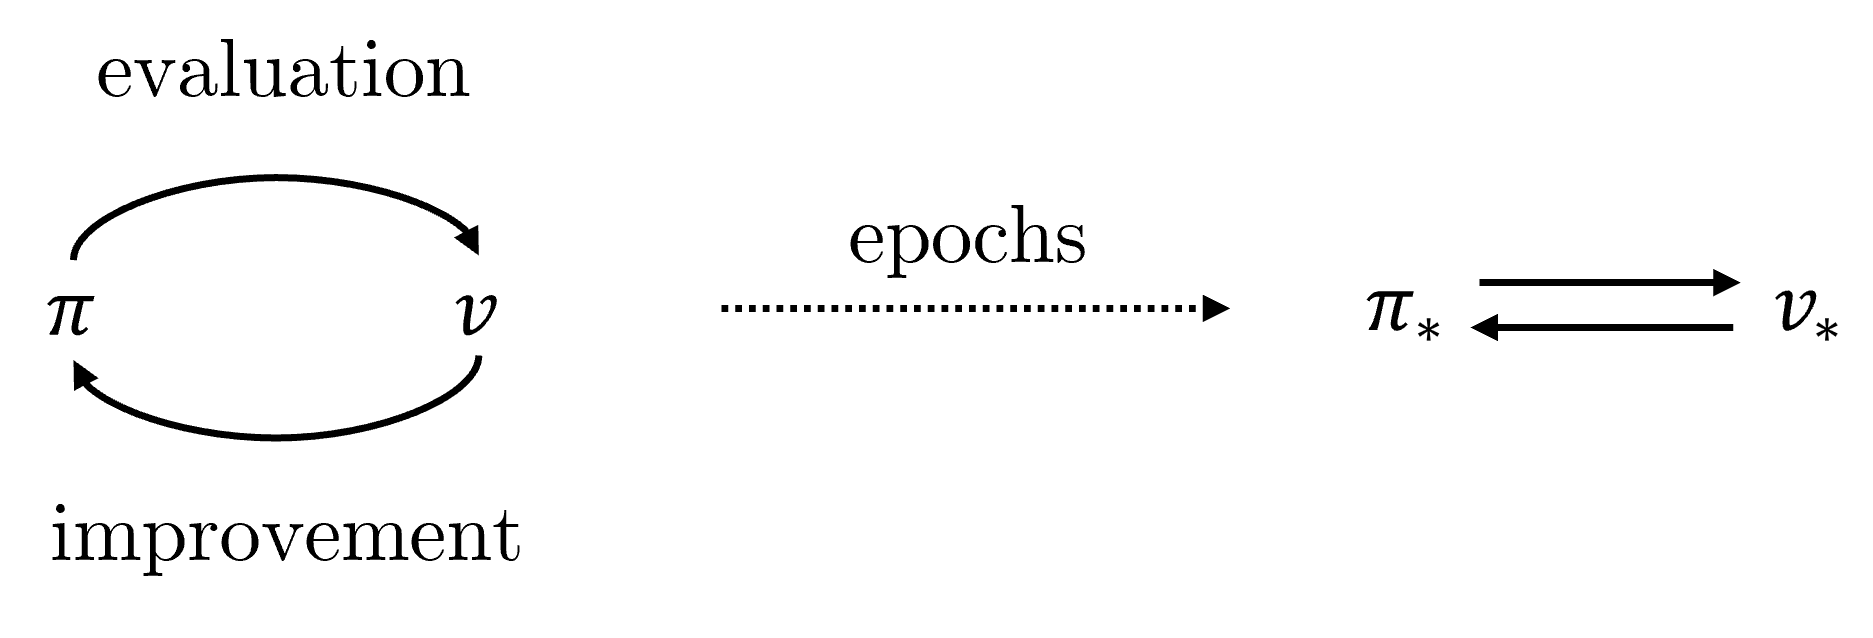
\includegraphics[width=0.5\linewidth]{figures/background/PolicyIterationConcept.png}
        \caption[Policy iteration concept]{Policy iteration concept. We can see the alternating uptate between policy and value-function. This process continues until we reached either the optimal policy and optimal value-function or is limited by the number of epochs. Adapted graphic from~\cite{SuttonBartoRLBook}}
        \label{fig:policy-iteration-concept}
    \end{center}
\end{figure}

We can also think about this process as a tradeoff between improving the policy towards an optimal greedy behavior which makes the value function incorrect (blue arrows indicate a policy improvement step) and adapting the value function with respect to the current policy which makes the policy automatically less optimal (red arrows indicate a policy evaluation step). Despite this tradeoff the algorithm tends to find an optimal solution for the policy and the value function in the long run~\cite{SuttonBartoRLBook}.

% \begin{figure}
    \begin{center}
        
\includegraphics[width=0.5\linewidth]{figures/place_holder.png}
        \caption[policy iteration funnel]{Figure shows the policy iteration funnel. The red arrows are a symbolic policy improvement step which is moving away from a precise value function. The blue arrows are a symbolic policy evaluation step which is moving the current policy further away from a greedy and thus stable policy. Both criterions are moving over time closer together until convergence with the optimal policy $\pi_*$ and the optimal value function $v_*$}
        \label{fig:policy-iteration-concept-funnel}
    \end{center}
\end{figure}
\begin{figure}
    \begin{center}
        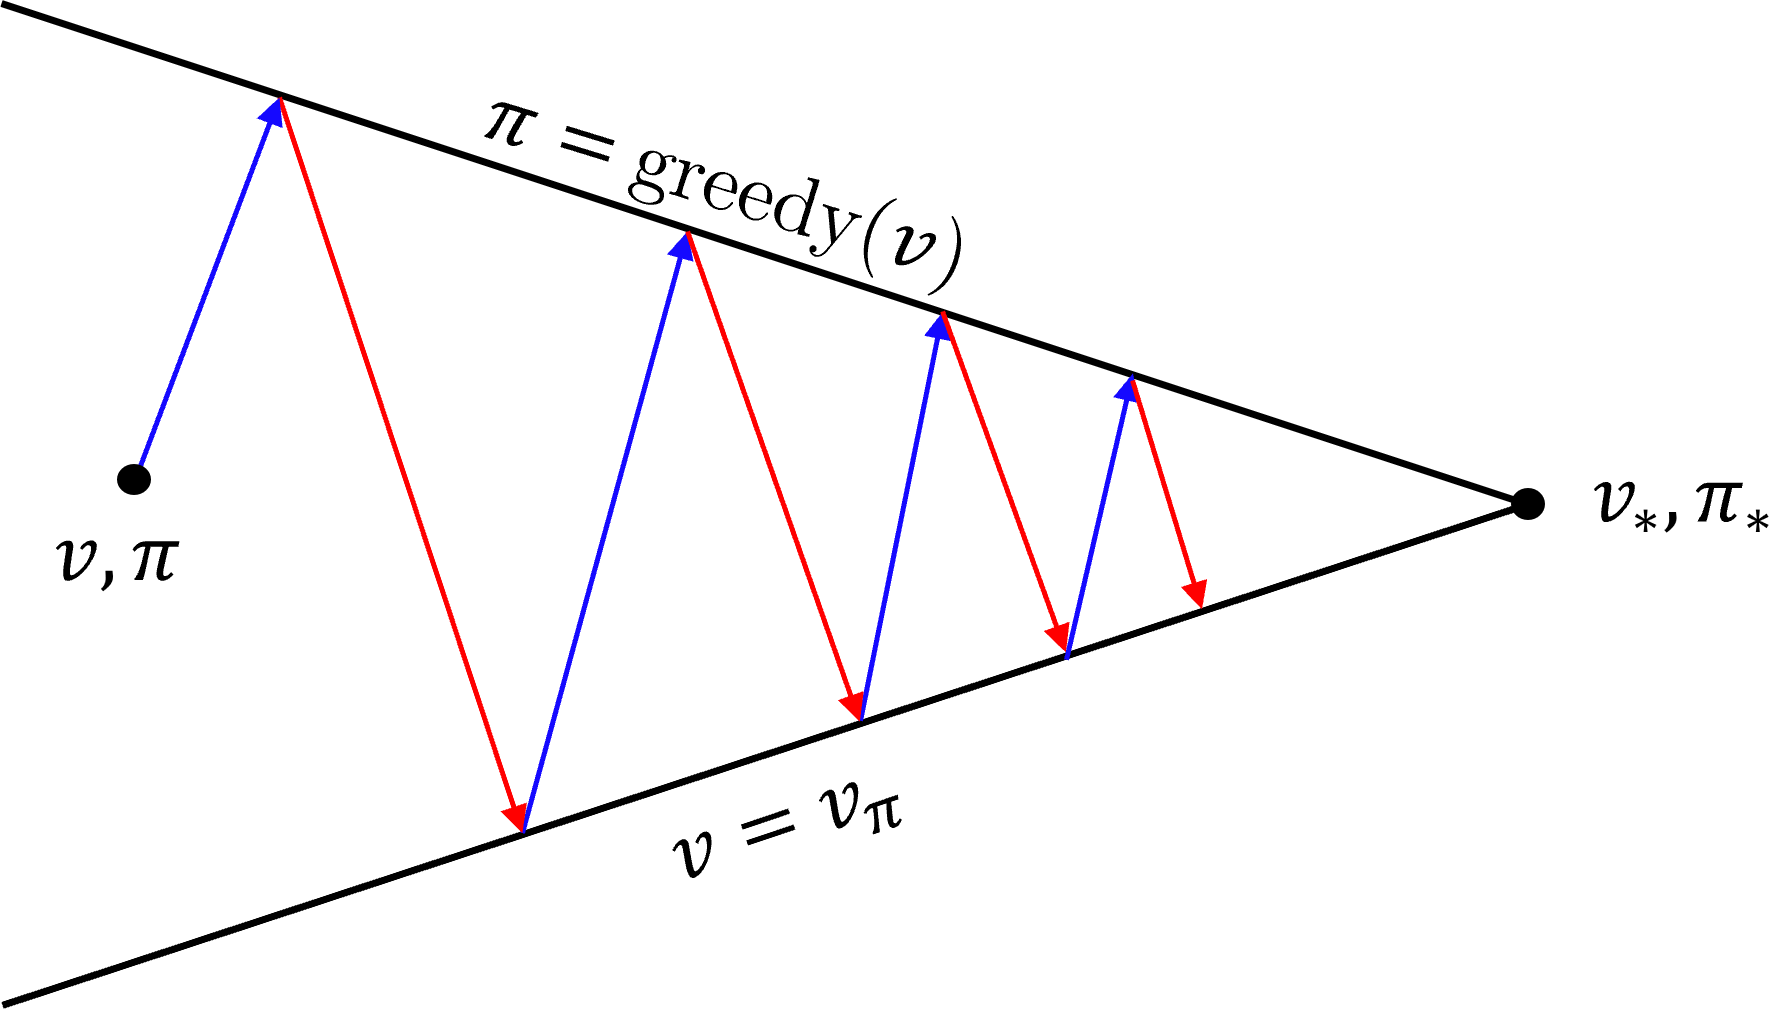
\includegraphics[width=0.5\linewidth]{figures/background/PolicyIterationFunnel.png}
        \caption[Policy iteration funnel]{Policy iteration funnel. The red arrows are a symbolic policy improvement step which is moving away from a precise value function. The blue arrows are a symbolic policy evaluation step which is moving the current policy further away from a greedy and thus stable policy. Both criterions are moving over time closer together until convergence with the optimal policy $\pi_*$ and the optimal value function $v_*$. Figure was adapted from~\cite{SuttonBartoRLBook}}
        \label{fig:policy-iteration-concept-funnel}
    \end{center}
\end{figure}

\section{Soft Actor Critic}\label{sec:SAC}
% Briefly explain what the SAC algorithm is and why it is important
% Provide a preview of what the chapter will cover

Soft Actor-Critic was introduced by Tuomas Haarnoja, Aurick Zhou, Pieter Abbeel and
Sergey Levine in 2018 in their paper: ``Soft Actor-Critic: Off-Policy Maximum Entropy Deep Reinforcement Learning
with a Stochastic Actor''~\cite{SAC_Paper}. It is an algorithm belonging to the family of model free, off-policy, actor-critic reinforcement learning algorithms. The family of actor-critic algorithms addresses challenges in exploration and sample efficiency. Similar to  other actor-critic algorithms it also employs the alternating concept of a policy improvement step and a policy evaluation step. In contrast to other actor-critic algorithms like deep deterministic policy gradient (DDPG) from~\cite{DPG_Paper}~\cite{DDPG_Paper} it uses the concept of entropy regularization and uses a stochastic policy for promoting exploration in the reinforcement learning environment. 
By jointly optimizing the policy and value functions using the maximum entropy objective enabled by entropy regularized, SAC effectively explores the environment while seeking to maximize rewards. This approach results in robust and adaptive policies that can efficiently handle various RL tasks also shown by Tuomas Haarnoja et al.~\cite{SAC_Applications_Paper}

In this section will introduce the concept of actor-critic algorithms, provide a detailed description of the SAC algorithm architecture, including entropy regularization and explain how to train the algorithm under the maximum entropy objective. 

\subsection{Actor-Critic Algorithms}

% Describe the basic actor-critic architecture and its limitations
% Explain the difference between on-policy and off-policy learning
% Describe the advantage of using a critic in the actor-critic algorithm
The basic actor-critic architecture is a type of reinforcement learning algorithm that consists of two components: an actor and a critic~\cite{Actor_Critic_Algorithms}. The actor also referred to as the policy $\pi_\theta$ is responsible for selecting actions based on the current state, while the critic also referred to as a value function $v_{\pi_\theta}$ or a state value function $q_{\pi_\theta}$, evaluates the quality of the actors actions by estimating the expected return. Like as introduced in \secref{sec:Generalized-Policy-Iteration} the actor uses the feedback from the critic to adjust its policy and improve its performance.

One additional factor to distinguish between reinforcement learning is by either on-policy learning or off-policy learning as in~\cite{SuttonBartoRLBook}. \\
On-policy learning or off-policy learning refer to different methods for updating the policy in reinforcement learning. In on-policy learning, the agent learns from the data generated by its current policy, while in off-policy learning, the agent learns from data generated by a different policy. On-policy learning can be more stable, but it may require more data to converge. Off-policy learning can be more efficient, but it can be more sensitive to the quality of the data.

The advantage of using a critic in the actor-critic algorithm is: it provides a more stable feedback signal than using only rewards~\cite{SpinningUp2018}. The critic estimates the expected return from a state, for the value function, or a state action pair for the action-value function, which takes into account the long-term consequences of actions. This allows the actor to learn from the critics feedback and improve its performance more efficiently than if it only received reward signals. % Additionally, the critic can help to generalize across different states and actions, improving the overall performance of the algorithm~\cite{SpinningUp2018}.

One limitation of the basic actor-critic architecture is that it can suffer from high variance and slow convergence due to the interaction between the actor and critic. This can be addressed through the use of techniques such as baseline subtraction and eligibility traces~\cite{SpinningUp2018}~\cite{SuttonBartoRLBook}.

Popular examples for actor critic algorithms are:
\begin{itemize}
	\item Deep Deterministic Policy Gradient presented by Timothy P. Lillicrap et al.~\cite{DDPG_Paper}
	\item Soft Actor-Critic presented by Tuomas Haarnoja~\cite{SAC_Paper}
	\item Asynchronous advantage actor critic (A3C) presented by Volodymyr Mnih et al.~\cite{A3C_Paper}
\end{itemize}


% Explain the concept of entropy regularization and its role in the SAC algorithm
% Describe the architecture of the SAC algorithm and how it differs from traditional actor-critic algorithms
% Explain how the actor and critic are trained using the maximum entropy objective
% Discuss the advantages of the SAC algorithm, such as improved sample efficiency and exploration

\subsection{Entropy Regularization}\label{sec:entropy-regularization}

Entropy regularization is a policy regularization technique by incorporating the policy entropy, used to encourage the policy to explore a diverse range of actions during training. In SAC, entropy regularization is achieved by adding the entropy $H(\pi_\theta)$ as in~\eqref{eqn:policy-entropy} to the policy objective function in~\eqref{eqn:policy-update} from~\cite{SuttonBartoRLBook}.

\begin{align}\label{eqn:policy-entropy}
    \mathrm{H}(\pi_\theta) &:= \underset{s\sim \mathcal{D}}{\mathbb{E}}\left[\mathrm{H}(\pi_\theta(\cdot|s))\right] \nonumber\\
    &=\underset{s\sim\mathcal{D}, a\sim\pi_\theta(\cdot|s)}{\mathbb{E}}\left[- \log(\pi_\theta(a|s))\right]
\end{align} 

Including entropy into the objective function encourages the policy to generate actions with higher entropy (higher randomness), leading to more exploration, possibly accelerate training and preventing converging to a poor local optimum~\cite{SpinningUp2018}.

The randomness or uncertainty of a policy for a given state action pair $\pi_\theta(a|s)$ can be computed  by seeing  $\pi_\theta(a|s)$ as a density function and taking $\pi_\theta(\cdot|s) = \mathcal{N}\left(\mu(\pi_\theta(\cdot|s)), \sigma(\pi_\theta(\cdot|s))\right)$ as a parameterized normal distribution from which the action $a \sim \pi_\theta(\dot|s)$ is sampled. Therefor it possible to acquire the probability $\pi_\theta(a|s)$ of an action $a$ with as in~\eqref{eqn:Gauss-Prob-Policy}.

\begin{align}
	\pi_\theta(a|s) = \frac{1}{\sigma(\pi_\theta(\cdot|s)) \sqrt{2\pi}} \exp\left(-\frac{1}{2}\frac{(a -\mu(\pi_\theta(\cdot|s)))^2}{\sigma(\pi_\theta(\cdot|s))^2}\right) \label{eqn:Gauss-Prob-Policy}
\end{align}

As a result of entropy regularization in each time step both value function $v_{\pi_\theta}$ and action-value function $q_{\pi_\theta}$ become affected and turn into their counterpart $v_{\pi_\theta, H}$ and $q_{\pi_\theta, H}$ in~\eqref{eqn:valuefunction-entropy-reg} and~\eqref{eqn:action-valuefunction-entropy-reg} below.  Note that~\eqref{eqn:action-valuefunction-entropy-reg-recursive} is the recursive version of~\eqref{eqn:action-valuefunction-entropy-reg}.

\begin{align}
	v_{\pi_\theta, H}(s) &= \underset{\tau\sim\pi_\theta}{\mathbb{E}}\left[\sum_{t=0}^T\gamma^t\left(R_t + \alpha H(\pi_\theta(\cdot|s_t))\right)\mid s_0 = s\right]\label{eqn:valuefunction-entropy-reg} \\
	q_{\pi_\theta, H}(s, a) &= \underset{\tau\sim\pi_\theta}{\mathbb{E}}\left[\sum_{t=0}^T\gamma^t R_t + \alpha \sum_{t=1}^T \gamma^t H(\pi_\theta(\cdot|s_t))\mid s_0 = s, a_0=a\right]\label{eqn:action-valuefunction-entropy-reg} \\
	&= \underset{s'\sim P, a' \sim \pi_\theta}{\mathbb{E}}\left[R_t + \gamma (q_{\pi_\theta, H}(s', a') + \alpha H(\pi_\theta(\cdot|s')))\right]\label{eqn:action-valuefunction-entropy-reg-recursive} 
\end{align} \todo{include entropy in the first time step -> look at the code and search for the appropriate paper}

This changes subsequently also the original relation between $v_{\pi_\theta}$ and $q_{\pi_\theta}$. $v_{\pi_\theta, H}$ and $q_{\pi_\theta, H}$ are connected via~\eqref{eqn:valuefunction-action-valuefucntion-reg-connection}.

\begin{equation}\label{eqn:valuefunction-action-valuefucntion-reg-connection}
	v_{\pi_\theta, H}(s) = \mathbb{E}_{\pi_\theta}\left[q_{\pi_\theta}(s, a)\right] + \alpha H(\pi_\theta)
\end{equation} \todo{proof in appendix?}

Note, that we introduce a new parameter $\alpha$ into $v_{\pi_\theta,H}$ and $q_{\pi_\theta,H}$. This parameter controls the tradeoff between exploration and exploitation.  Higher values of $\alpha$ promote more exploration, whereas lower values of $\alpha$ encourage more exploitation in the Soft Actor-Critic algorithm~\cite{SpinningUp2018}. For more details how to this parameter is used in Soft Actor-Critic please have look into \secref{sec:SAC-architectur}.

For simplification we will now refer to the entropy regularized value function $v_{\pi_\theta,H}$ as $v_{\pi_\theta}$ and action-value-function $q_{\pi_\theta,H}$ as $q_{\pi_\theta}$. 

This change also influences the original reinforcement learning problem as stated in~\eqref{eqn:RL-policy-valuefunction} and converts it into~\eqref{eqn:RL-policy-problem-reg}. Due to the stated relation between regularized value-function and regularized action-value-function as in~\eqref{eqn:valuefunction-action-valuefucntion-reg-connection} we can make the optimization problem independent from the value-function and get~\eqref{eqn:RL-policy-problem-reg-action-value-function}.

\begin{align}
	\pi_\theta^* &= \arg \max_{\pi_\theta} v_{\pi_\theta,H} \nonumber \\
	&\overset{\mathclap{\strut(\ref{eqn:RL-policy-valuefunction})}}{=} \arg \max_{\pi_\theta} \mathbb{E}_{\pi_\theta}\left[\sum_{t=0}^T \gamma^t \left(R_t + \alpha H(\pi_\theta)\right)\mid S_t = s\right] \label{eqn:RL-policy-problem-reg} \\
	&\overset{\mathclap{\strut(\ref{eqn:valuefunction-action-valuefucntion-reg-connection})}}{=} \arg \max_{\pi_\theta} \mathbb{E}_{\pi_\theta}\left[q_{\pi_\theta}(s, a)\right] + \alpha H(\pi_\theta) \nonumber \\
	&\overset{\mathclap{\strut(\ref{eqn:policy-entropy})}}{=}\arg \max_{\pi_\theta} \mathbb{E}_{\pi_\theta}\left[q_{\pi_\theta}(s, a) - \alpha \log \pi_\theta(a|s)\right]\label{eqn:RL-policy-problem-reg-action-value-function}
\end{align}

\subsection{Algorithm Architecture}\label{sec:SAC-architectur}

In contrast to other actor-critic algorithms like: DDPG~\cite{DDPG_Paper} or A3C~\cite{A3C_Paper} SAC learns additional to a parameterized policy $\pi_\theta$, two critics in the form of two parametrized $q$ functions $Q_{\phi_0}$ and $Q_{\phi_1}$ as well as their corresponding target functions $Q_{\phi_{\text{target}, 1}}$ and $Q_{\phi_{\text{target}, 1}}$. The usage of target action-value functions enhances the accuracy of the estimates and contributes to a more stable learning process~\cite{SAC_Applications_Paper}.

Further SAC utilizes a stochastic policy, which means that the policy outputs a parameterized probability distribution over actions instead of directly selecting deterministic actions and optionally adding noise on top. This stochastic nature allows SAC to capture the exploration-exploitation trade-off directly within the policy.
The training process in SAC is based on the maximum entropy objective~\cite{SpinningUp2018}. Its goal is to find a policy that maximizes the cumulative reward~\eqref{eqn:discounted-cumulative-return} and the maximum entropy~\eqref{eqn:policy-entropy}. Fortunately, we have derived an entropy regularized value-function and action-value-function in \secref{sec:entropy-regularization} and are able to use those definition to derive loss functions for actor and critic based on the maximum entropy objective. 

Because we will have a closer look into actual implementation, we now refer to the action-value-function as their parameterized approximations $Q_{\pi_i}$.

To \textbf{train the parameterized action-value-functions} the objective function (\ref{eqn:q-loss}) is defined as the expected squared difference between the action-state-value $Q_{\phi_i}(s, a)$ and its temporal difference target $y(r, s', d)$.~\eqref{eqn:q-loss} leads directly to the update equation (\ref{eqn:q-update}) as its derived empirical counterpart.

\begin{equation}\label{eqn:q-loss}
	\mathcal{L}_Q(\phi_i, \mathcal{D}) = \mathbb{E}_\mathcal{D}\left[\left(Q_{\phi_i}(s, a) - y(r, s', d)\right)^2\right]
\end{equation}

The temporal difference target target $y$ is defined as in~\eqref{eqn:td-target} with $\hat{a}' \sim \pi\theta(\cdot| s')$. To stabilize the target signal SAC applies the clipped double-Q trick, where it selects the minimum q-value between the two target q-functions $Q_{\phi_{\text{target}, i}}$.

\begin{equation}\label{eqn:td-target}
	y(r, s', d) = r + \gamma(1 - d) \left(\min_{j=0,1}Q_{\phi_{\text{target}, i}}(s', \hat{a}') - \alpha \log \pi_\theta(\hat{a}'| s')\right)
\end{equation} \todo{where exactly is the target coming from?}

This function is employed in the SAC algorithm in~\eqref{eqn:td-target-batch} but with the small difference that all arguments are sampled from a minibatch $\mathcal{B}$. 

To \textbf{train the policy} we are required to use the reparameterization trick to be able to differenciate the parameterized policy $\pi_\theta$~\cite{ReparameterizationTrick}.
This process transforms the action $\hat{a}$ sampled from the policy into the function as specified in~\eqref{eqn:reparameterization-trick}. 

\begin{equation}\label{eqn:reparameterization-trick}
	\hat{a}_\theta(s, \epsilon) = \tanh(\mu(\pi_\theta(\cdot|s)) + \sigma(\pi_\theta(\cdot|s)) \bigodot \epsilon), \ \epsilon \sim \mathcal{N}(0, I)
\end{equation}

Within the reparameterization of an action we also bound it into a finite range of $(-1, 1)$. This has the advantage bounding actions to standardized limits reducing the risk of undesirable or catastrophic action outcomes. Since we squash the actions with $\tanh$ we also have to adapt the log-likelihood $\log \pi_\theta(a|s)$ of an action into:

\begin{equation*}
	\log \pi_\theta(a|s) = \log \pi_\theta(a|s) - \sum_{i=1}^{|\mathcal{A}|} \log(1 - \tanh(\hat{a}_\theta(s, \epsilon))), \ \epsilon \sim \mathcal{N}(0, I)
\end{equation*}

For more details please refer to~\cite{SAC_Applications_Paper}.

To compute the policy loss, as in training the action-value-function approximation, the crucial step involves replacing $q_{\pi_\theta}$ with one of our function approximators $Q_{\phi_i}$. SAC utilizes the minimum of the two $q_{\pi_\theta}$ approximators $\min_{i=0,1} Q_{\phi_i}$. Consequently, the policy is optimized based on this minimum action-state-value approximation and therefor make only more conservative estimates.
\begin{equation}\label{eqn:policy-loss}
	\mathcal{L}_\pi(\theta, \mathcal{D}) = - \underset{s\sim\mathcal{D}, \epsilon\sim\mathcal{N}(0, I)}{\mathbb{E}}\left[\min_{i=0,1}Q_{\phi_i}(s, \hat{a}_\theta(s, \epsilon) - \alpha \log \pi_\theta(\hat{a}_\theta(s, \epsilon)| s))\right]
\end{equation}

Note that we are taking the negative expectation because we want to maximize the expected return and the entropy by using SGD as in~\eqref{eqn:policy-update} in \algoref{alg:SGD}. The different notation can be explained a ${\{s, a, r, s', d\}}_{\mathcal{B}, k}$ stand for the $k$th element from the minibatch $\mathcal{B}$..

Now lets turn to the entropy regularization parameter $\alpha$. In general there are two types of Soft-Actor-Critic implementations. One proposed by~\cite{SAC_Paper} and implemented in~\cite{stable-baselines3} treads $\alpha$ as constant parameter.  The optimal $\alpha$ parameter, leading to the most stable and rewarding learning, may vary across different environments, necessitating thoughtful tuning for optimal performance.
The second approach how to treat $\alpha$, proposed by~\cite{SAC_Applications_Paper}, adjusts $\alpha$ constantly during the training process. The optimization criterion is stated as:

\begin{equation}\label{eqn:alpha-criterion}
	\mathcal{L}_\alpha(\pi_\theta, \bar{H}) = \underset{a_t\sim\pi_\theta}{\mathbb{E}}\left[-\alpha \log \pi_\theta(a_t|s_t) - \alpha \bar{H}\right]
\end{equation}

\eqref{eqn:alpha-criterion} resembles an objective for dual gradient descent because we are trying to minimize $\alpha$ but also the expected difference between the policy entropy and a target entropy $\bar{H}$ as a hyperparameter. In practice this can be translated into a positive gradient if the expected difference is positive so the agent is less exploring as should be and into a negative gradient if the difference is negative so the agent is to focused on exploring. Selecting a target entropy is not as delicate as selecting a fixed $\alpha$ because you are able to read from training results if your environment requires a more or less greedy policy~\cite{SpinningUp2018}.

\begin{algorithm}
	\caption{Soft Actor Critic}\label{alg:SAC}
	\begin{algorithmic}
		\State{} Input: initial policy parameters $\theta$, Q-function parameters $\phi_0$, $\phi_1$, empty replay buffer $\mathcal{D}$
			\State{} Set target parameters equal to main parameters $\phi_{\text{target}, 0}$ $\leftarrow$ $\phi_0$, $\phi_{\text{target}, 1}$ $\leftarrow$ $\phi_1$ 
			\For{$i$ in number of epochs}
			\State{} $s$ $\leftarrow$ reset environment
			
			\For{$t$ number of timesteps}
			\State{} $a$ $\sim$ $\pi_\theta(\cdot | s)$
			\State{} $s'$, $r$, $d$ $\leftarrow$ execute $a$ in environment
			\State{} Store $(s, a, r, s', d)$ in replay buffer $\mathcal{D}$
			\If{$d$ is true}
			\State{} break and reset environment
			\EndIf{}
			\State{} $s$ $\leftarrow$ $s'$
			\EndFor{}
			
			\If{$|\mathcal{D}|$ > minimal buffer size}
			\For{number of train iterations}
			\State{} sample minibatch: $(s_\mathcal{B}, a_\mathcal{B}, r_\mathcal{B}, s'_\mathcal{B}, d_\mathcal{B}) = \mathcal{B}$ $\leftarrow$ $\mathcal{D}$ 
			\State{} compute td target $y$ with $\tilde{a}'_\mathcal{B} \sim \pi_\theta(\cdot|s'_\mathcal{B})$
			\begin{equation}\label{eqn:td-target-batch}
				y(r_\mathcal{B}, s'_\mathcal{B}, d_\mathcal{B}) = r_\mathcal{B} + \gamma(1 - d_\mathcal{B}) \left(\min_{j=0,1}Q_{\phi_{\text{target}, i}}(s'_\mathcal{B}, \hat{a}'_\mathcal{B}) - \alpha \log \pi\theta(\hat{a}'_\mathcal{B}| s'_\mathcal{B})\right)
			\end{equation}
			\State{} Update Q-functions for parameters $\phi_i$ $i \in \{0, 1\}$ using:
			\begin{equation}\label{eqn:q-update}
				\nabla_{\phi_i} \frac{1}{|B|} \sum_{k \in |\mathcal{B}|}\mathcal{L}_Q(\phi_i, \mathcal{D})   
			\end{equation}
			\State{} Update policy using:
			\begin{equation}\label{eqn:policy-update}
			   \nabla_{\theta} \frac{1}{|\mathcal{B}|}\sum_{k \in |\mathcal{B}|}\mathcal{L}_\pi(\theta, \mathcal{D})
			\end{equation}
			\State{} Update $\alpha$ with target entropy $H_\text{target}$ and $\tilde{a}_\mathcal{B} \sim \pi_\theta(\cdot|s_\mathcal{B})$ using:
			\begin{equation*}
				\nabla_\alpha -\frac{\alpha}{|\mathcal{B}|} \sum_{k \in |\mathcal{B}|} \mathcal{L}_\alpha(\pi_\theta, \bar{H})
			\end{equation*}
			\State{} Update target networks $\phi_{\text{target}, i}$ $i \in \{0, 1\}$ with $\phi_i$ $i \in \{0, 1\}$ using:
			\begin{equation*}
				\phi_{\text{target}, i} \leftarrow \rho \phi_{\text{target}, i} + (1 - \rho) \phi_i
			\end{equation*}
			\EndFor{}
			\EndIf{}
			\EndFor{}
	\end{algorithmic}
\end{algorithm}

\todo{rework equations from pseudo code}

\subsection{Advantages}

SAC offers several advantages over other actor-critic algorithms. Firstly, the entropy regularization leads to improved exploration, enabling the agent to efficiently explore its environment and discover optimal or near-optimal solutions~\cite{SAC_Paper}. Secondly, by encouraging stochastic policies, SAC provides more robust and adaptive policies that can handle uncertainties and variations in the environment.

Moreover, the SAC algorithm exhibits enhanced sample efficiency, meaning that it requires fewer interactions with the environment to learn effective policies~\cite{SAC_Applications_Paper}. The utilization of two critics $Q_{\phi_0}$ and $Q_{\phi_1}$ further contributes to a more stable learning process and can mitigate the issues of overestimation bias, leading to more accurate value estimates~\cite{SAC_Paper}.

\subsubsection{Applications}

% Provide examples of real-world applications of the SAC algorithm, such as robotics and game playing
% Explain how the SAC algorithm can be used in continuous action spaces
% Describe the limitations of the SAC algorithm and how they can be addressed

In robotics, the SAC algorithm has been used to control robots in tasks such as grasping objects, locomotion, and manipulation. The SAC algorithms ability to handle continuous action spaces makes it a suitable choice for robotic control, where fine-grained control is often required~\cite{SAC_Applications_Paper}.

In game playing, the SAC algorithm has been used to train agents to play video games such as Atari~\cite{SAC_Discrete_Paper}. The SAC algorithms ability to balance exploration and exploitation makes it effective in game playing, where agents must learn to navigate complex environments and respond to changing conditions~\cite{SAC_VideoGames_Paper}.

% \subsection{Extensions to SAC}
% 
% Describe extensions to the basic SAC algorithm, such as distributed SAC and multi-agent SAC
% Explain how SAC can be combined with other models, such as generative models

% \subsection{Current and Future Directions}
% 
% Describe current research trends in SAC, such as improving its performance in high-dimensional state spaces and addressing the issue of multi-task learning
% Discuss potential future applications of SAC, such as in healthcare and finance
% Explain challenges that must be addressed in order for SAC to continue to advance

% \subsection{Conclusion}
% 
% Summarize the main points of the chapter
% Emphasize the importance of SAC in a variety of fields
% Encourage further exploration of the topic.
 
\section{Neural Networks}

% Briefly explain what neural networks are and why they are important
% Provide a preview of what the chapter will cover. 

Neural networks are a class of artificial intelligence algorithms inspired by the structure and functioning of the human brain~\cite{DeepLearningTextBook}. \\
They consist of interconnected layers of artificial neurons that process and transform data. Neural networks are crucial in modern machine learning and deep learning applications due to their ability to learn complex patterns and representations from data, enabling them to solve a wide range of problems effectively~\cite{DeepLearningTextBook}.

In this chapter, we will delve into neural networks, looking at their evolution, architecture, training process and diverse applications.
% \subsection{Historical Overview}
% 
% Discuss the early history of neural networks, including the work of Warren McCulloch and Walter Pitts in the 1940s
% Explain how the field evolved in the 1950s and 1960s
% Discuss the challenges faced by researchers during this time, including the limitations of computing power and the lack of effective training algorithms

\subsection{The Rise of Deep Learning}

Neural networks were first invented in the 1940s and 1950s as a computational model inspired by the interconnected structure and functioning of the human brain, but their practical development was hindered by limitations in computing power and the lack of large datasets. 
The resurgence of interest in neural networks in the 2000s can be attributed to two major factors: the development of new algorithms and the availability of large datasets. Before the 2000s, neural networks faced limitations in training and optimization, hindering their effectiveness. However, new algorithms, such as the backpropagation algorithm and variants like stochastic gradient descent, emerged, making it feasible to train deeper networks efficiently. Additionally, advancements in computing power and the availability of vast datasets facilitated by the internet like image net~\cite{ImageNet} allowed neural networks to leverage big data for improved learning and performance~\cite{VGG16}~\cite{ResNet50}.

Nowadays neural networks are employed over a vast variety of tasks like image recognition~\cite{VGG16}, speech recognition~\cite{DL_SpeechRecognition}, natural language processing~\cite{DL_NLP} or robotics~\cite{DL_Robotics}. 
% Explain how the development of new algorithms and the availability of large datasets led to a resurgence in interest in neural networks in the 2000s
% Describe the key breakthroughs that made deep learning possible, including the development of convolutional neural networks and recurrent neural networks
% Provide examples of important applications of deep learning, such as image and speech recognition

\subsection{Neural Network Architecture}

% Explain the basic architecture of a neural network, including the role of input and output layers, hidden layers, and activation functions
% Describe different types of neural networks, including feedforward networks, recurrent networks, and convolutional networks
% Explain how neural networks can be trained using techniques such as backpropagation and stochastic gradient descent

Neural networks are a type of machine learning model inspired by the structure and function by the cell type of neurons. It consists like their biological model, of interconnected layers of individual units, called neurons~\cite{DeepLearningTextBook}.

The basic architecture of a neural network as in \figref{fig:neural_network_schema/feed-forward-architecture},  includes an input layer (yellow), one or more hidden layers (blue and green), and an output layer (red). The input layer receives the input data, which is then passed through the hidden layers before producing the output. Because the flow of information is only in the forward direction we call this basic architecture a feed forward neural network. The number of nodes in each layer and the connections between them are configured by the architecture of a network.
\begin{figure}
    \begin{center}
        \subfloat[Schematic drawing of a feed forward neural network.]{
            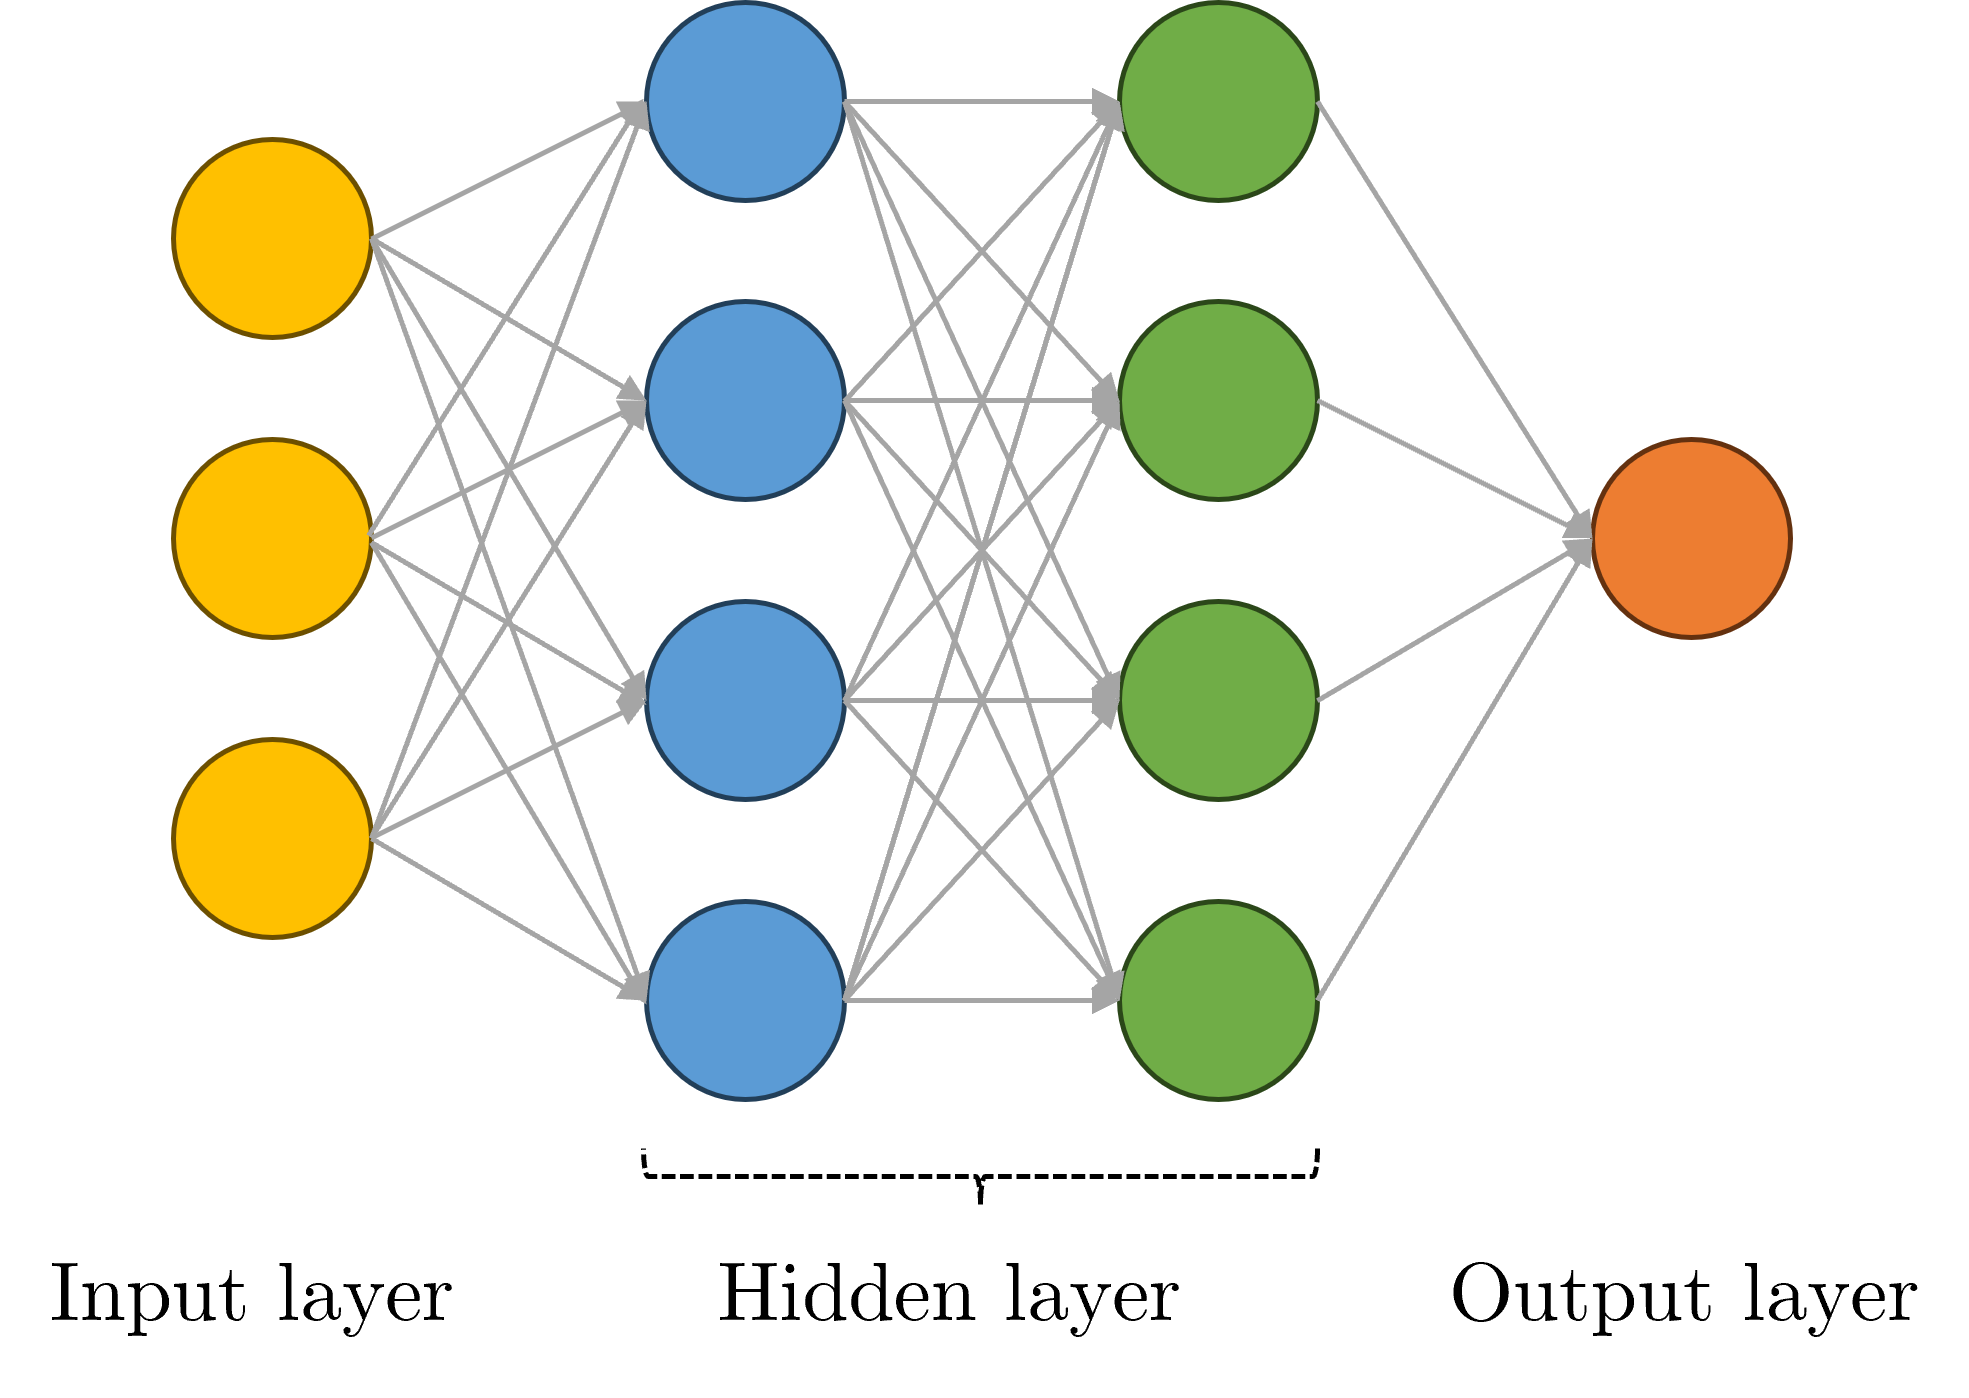
\includegraphics[width=0.51\linewidth]{figures/background/FeedForwardNetwork.png}
            \label{fig:neural_network_schema/feed-forward-architecture}
            }
        \hfill
        \subfloat[Schematic drawing of a single neuron.]{
            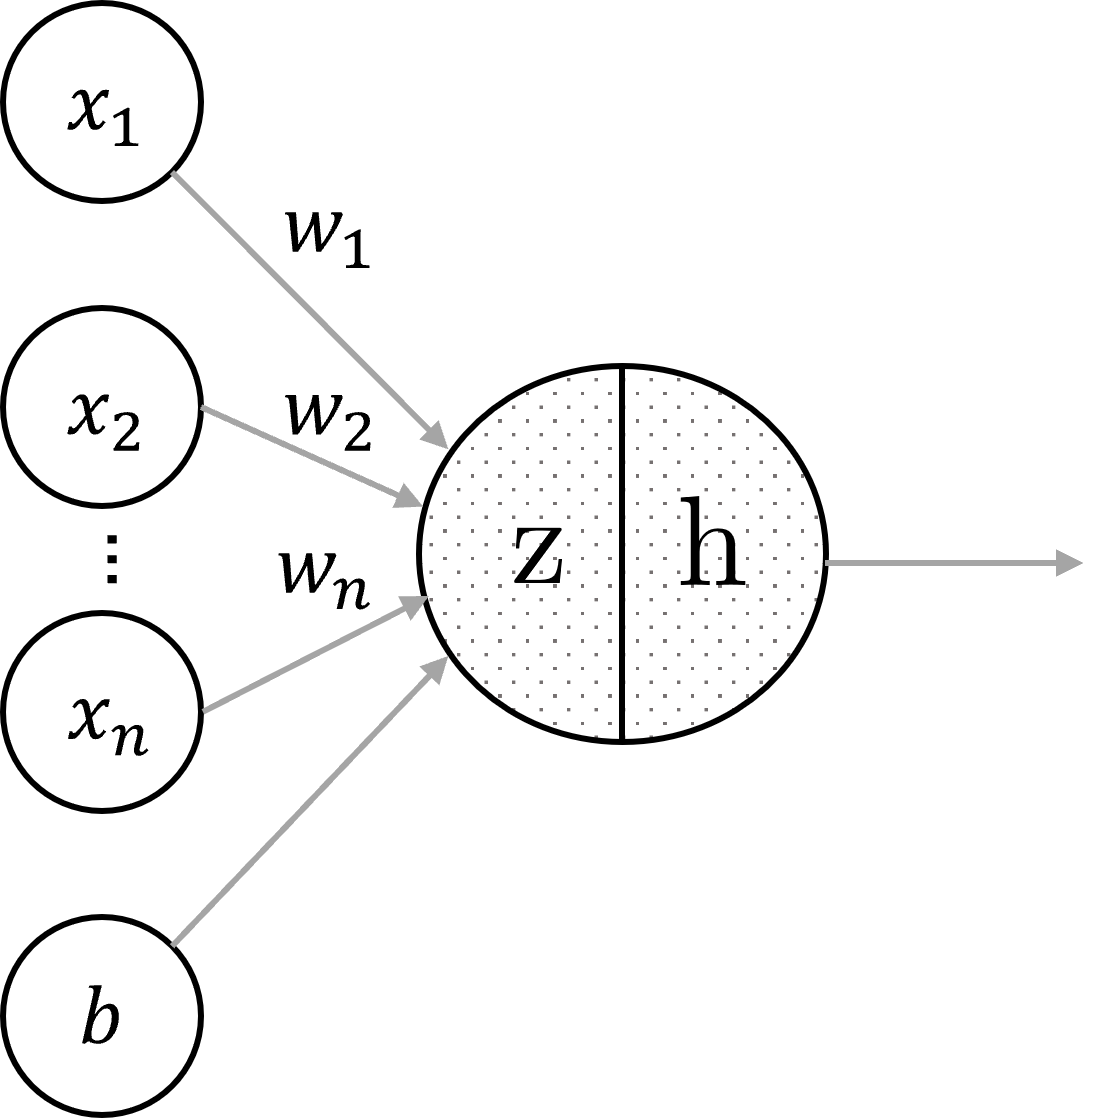
\includegraphics[width=0.35 \linewidth]{figures/background/Neuron.png}
            \label{fig:neural_network_schema/neuron}
            } 
    \end{center}
    \caption[Schematic architecture of neural network and neuron]{The figure shows the schematic drawing of a feed forward neural network and a neuron}
    \label{fig:neural_architecture}
\end{figure}

If we look at each individual neuron as in \figref{fig:neural_network_schema/neuron}, we can observe that each neuron is designed in the same way. First it calculates a weighted sum $z$ of its inputs $x$, the corresponding weights $w$ and bias $b$, before passing it into an activation function $h$ and finally passing the information to the next neuron. The activation function is designed to introduce nonlinearity into the model, allowing it to capture complex relationships between variables. Without a nonlinear activation function the whole network would be a single linear combination of its inputs and weights. Common activation functions include the sigmoid function~\cite{DL_ActivationFunctions}, the hyperbolic tangent function~\cite{DL_ActivationFunctions}, and the rectified linear unit (ReLU) function~\cite{DL_ReLU} as in \figref{fig:activation_function}.
\begin{figure}
    \begin{center}
        \subfloat[Sigmoid]{
            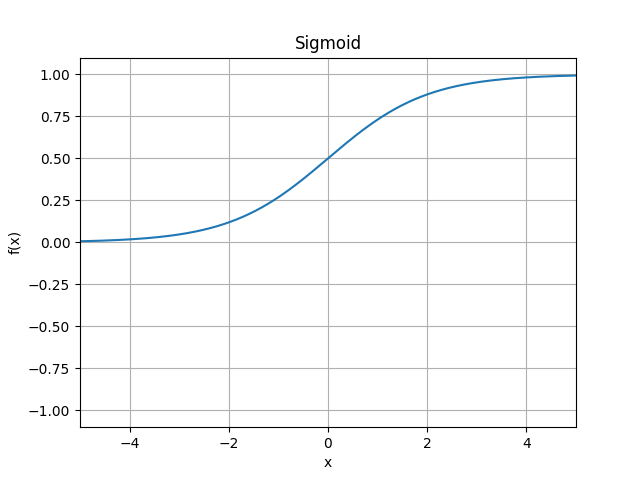
\includegraphics[width=0.315\linewidth]{figures/background/sigmoid.png}
            \label{fig:activation_function/sigmoid}
            }
        \hfill
        \subfloat[hyperbolic tangent function]{
            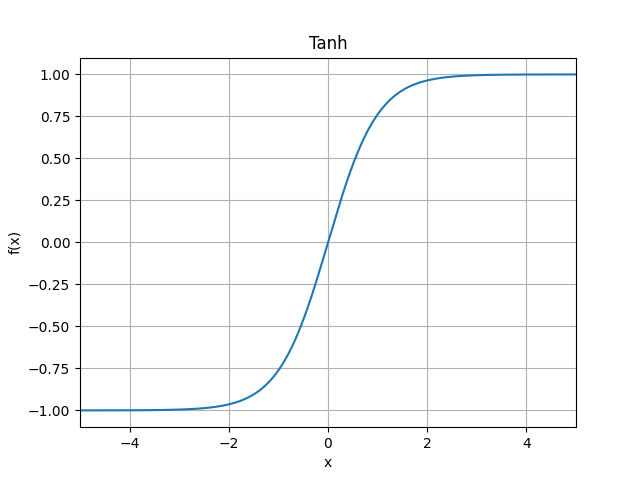
\includegraphics[width=0.315\linewidth]{figures/background/tanh.png}
            \label{fig:activation_function/tanh}
            }
        \hfill
        \subfloat[rectified linear unit]{
            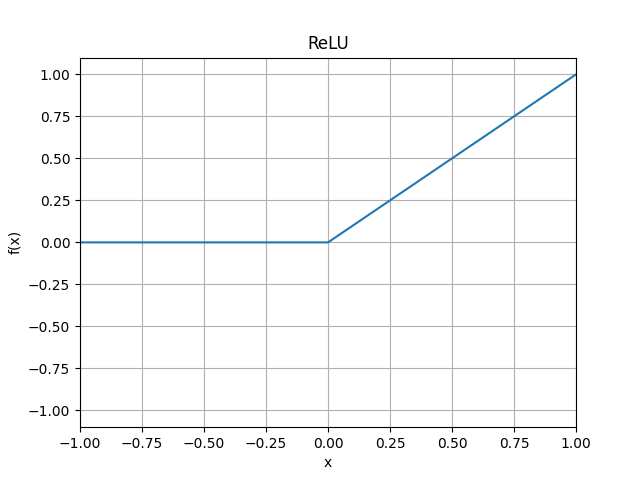
\includegraphics[width=0.315\linewidth]{figures/background/ReLU.png}
            \label{fig:activation_function/relu}
            }
    \end{center}
    \caption[common activation functions in a neural network]{common activation function for neural networks.}
    \label{fig:activation_function}
\end{figure}
\begin{figure}
    \begin{center}
        \subfloat[schematic drawing of convolutional neural network]{
            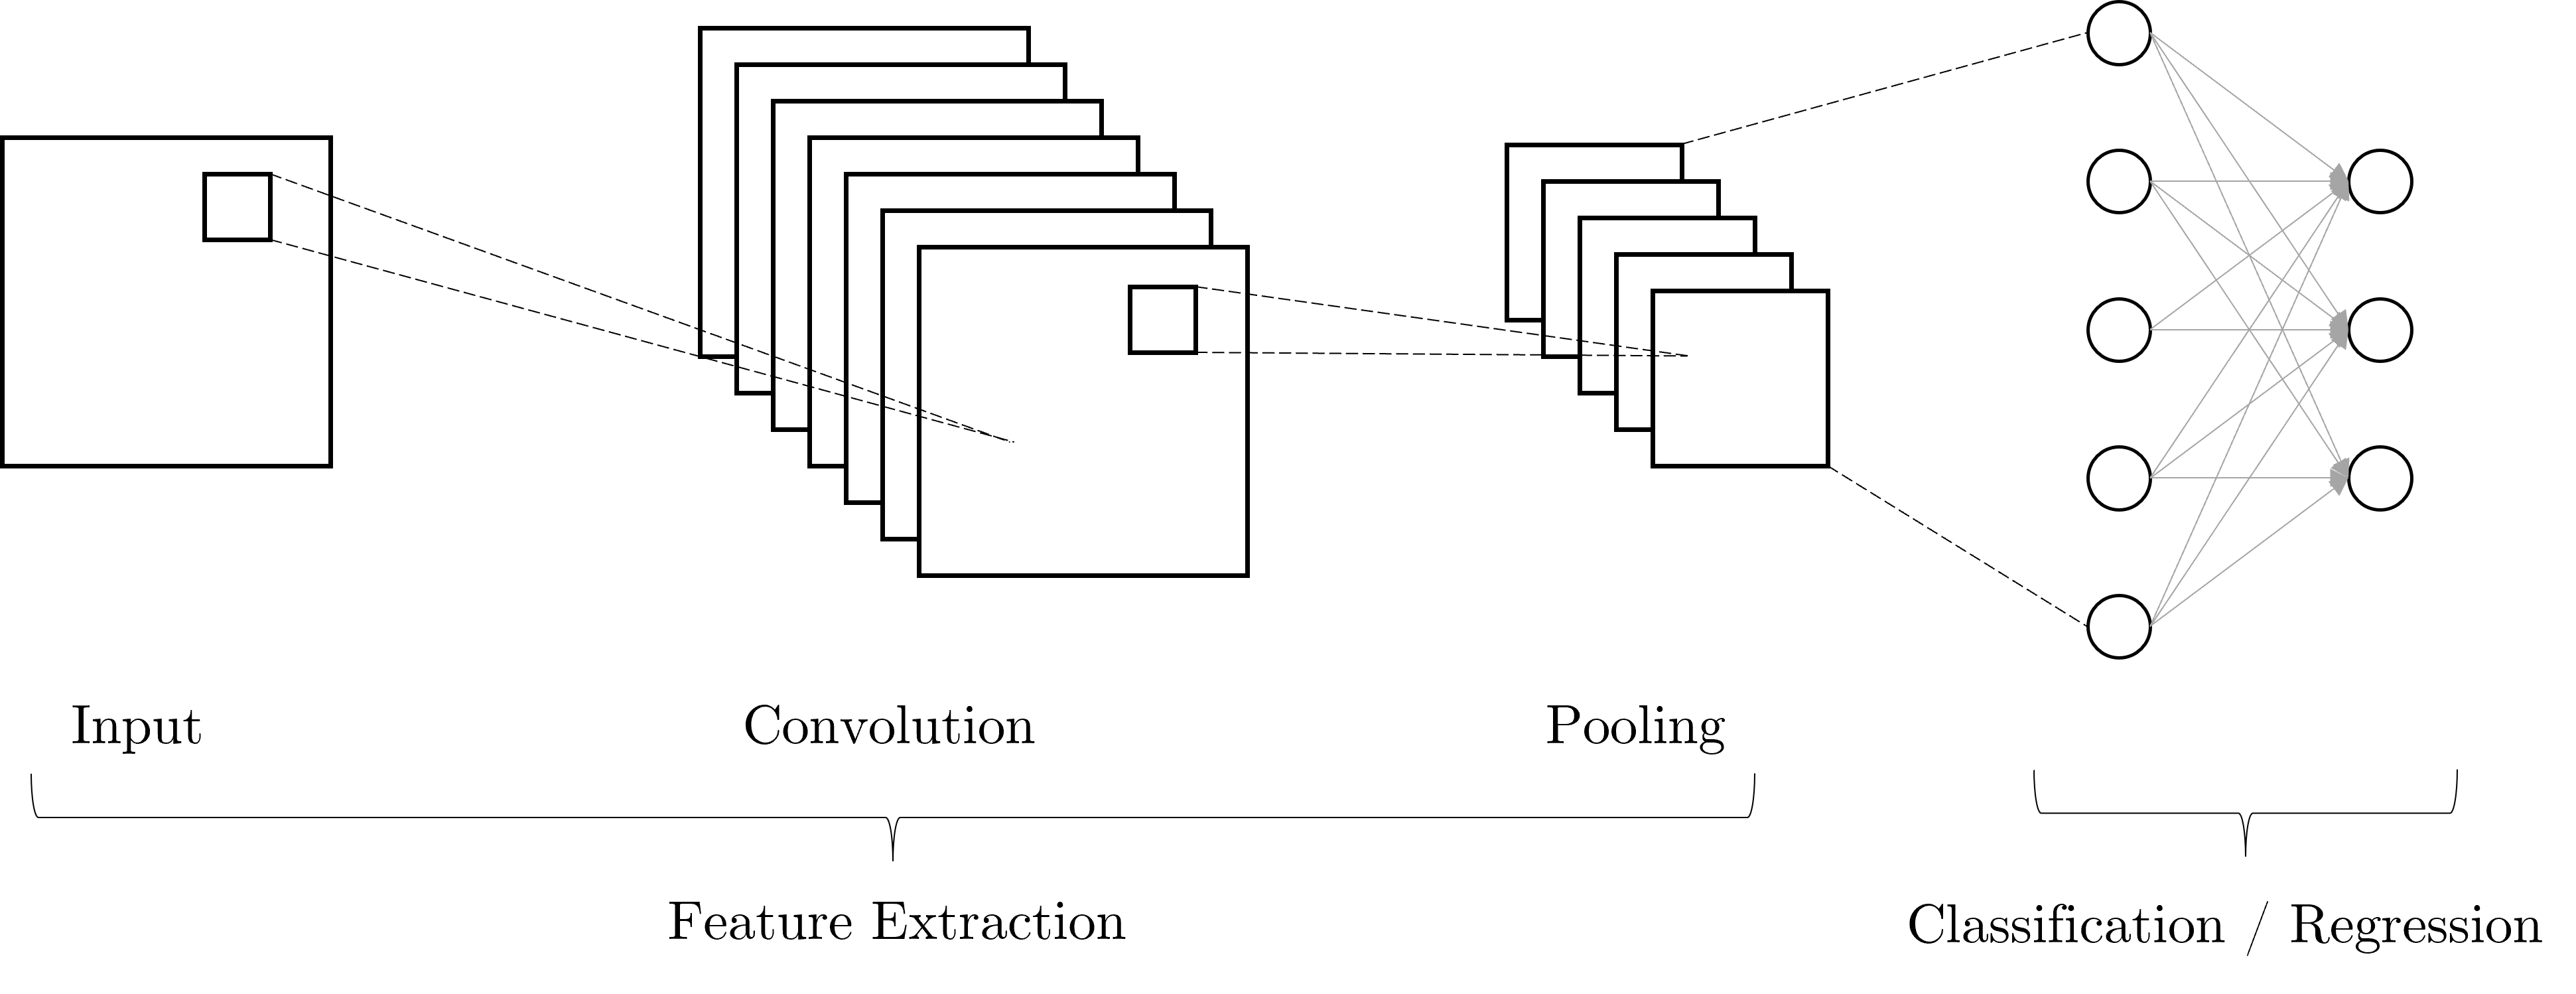
\includegraphics[width=0.7\linewidth]{figures/background/ConvNet.png}
            \label{fig:neural-network-architecture/convolutional-architecture}
            }
        \hfill
        \subfloat[schematic drawing of a recurrent neural network]{
            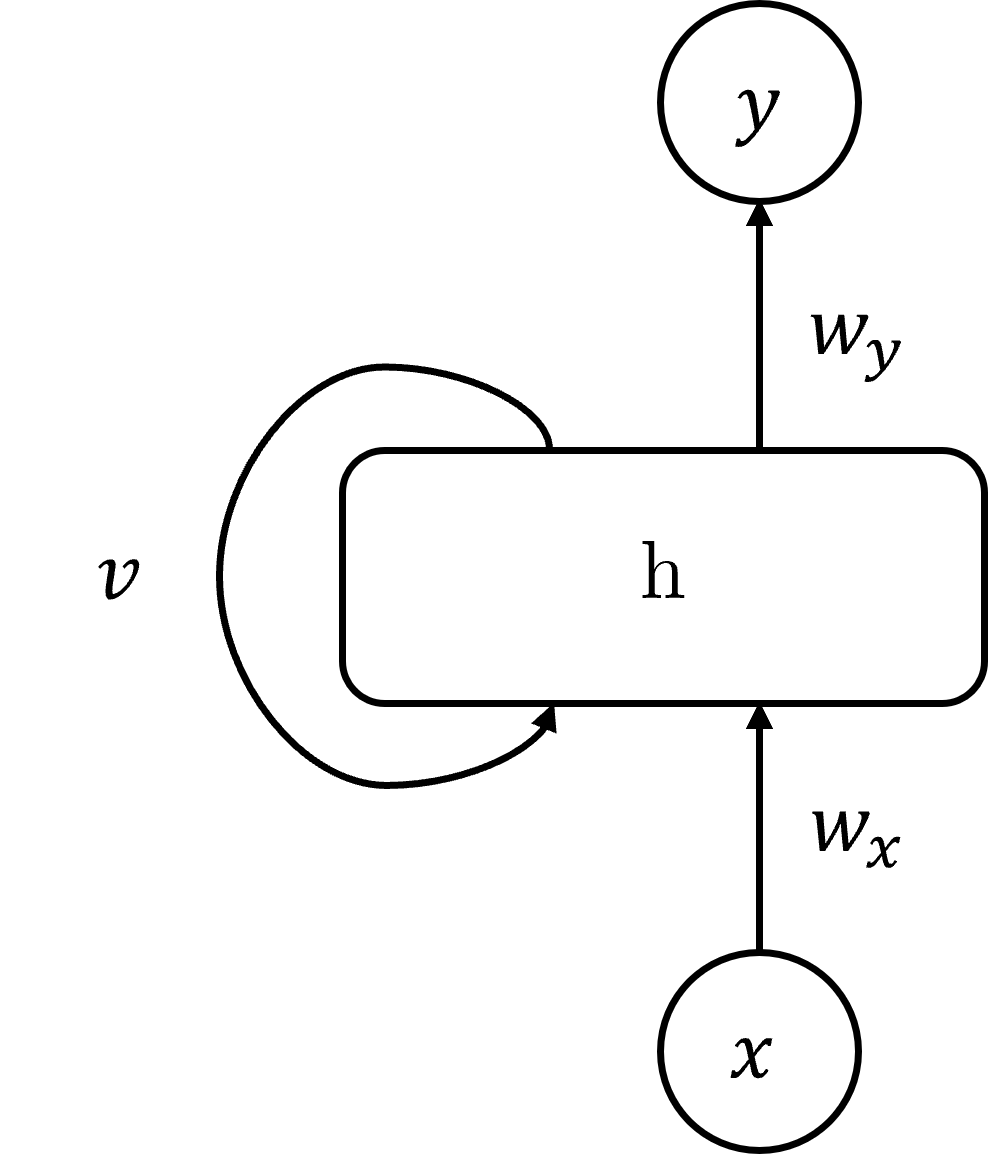
\includegraphics[width=0.2\linewidth]{figures/background/RNN.png}
            \label{fig:neural-network-architecture/recurrent-architecture}
            } 
    \end{center}
    \caption[advanced neural network architectures]{architecture of more advanced neural networks like the convolutional and the recurrent neural network}
    \label{fig:neural_network-architecture}
\end{figure}

There are several types of neural network architectures but most of them are based on following types: 
\begin{itemize}
	\item \textbf{Feedforward networks}~\cite{DL_FeedForward} as in \figref{fig:neural_network_schema/feed-forward-architecture} are the simplest type of neural network, consisting of a series of layers that process information in a single direction.
	\item \textbf{Convolutional networks}~\cite{DL_ConvNetwork} as in \figref{fig:neural-network-architecture/convolutional-architecture} are designed for image processing tasks and use convolutional layers to identify patterns and features within images. 
	\item \textbf{Recurrent networks}~\cite{DL_RecurrentNetwork} as in \figref{fig:neural-network-architecture/recurrent-architecture}allow information to be passed between nodes in a cyclical manner, making them suitable for processing sequential data. The development of Long Short-Term Memory (LSTM) and Gated Recurrent Unit (GRU) architectures further improved RNNs ability to model long-range dependencies.
\end{itemize}

\subsection{Train Neural Networks}

Neural networks are trained using techniques such as backpropagation~\cite{DL_Backpropagation} and stochastic gradient descent~\cite{SGD}~\cite{SGD2} as presented in \algoref{alg:SGD}. Backpropagation is an algorithm for calculating the gradient $\hat{g}$ of an optimization criterion with respect to the weights of the network. The gradient can then be used to update the weights and therefor improve the performance of the model with respect to the optimization function. A we can see in \algoref{alg:SGD} stochastic gradient descent minimizes the error presented by the optimization criterion by iteratively adjusting the weights based on randomly selected subsets of the training data. 

\begin{algorithm}
    \caption{Stochastic gradient descent}\label{alg:SGD}
    \begin{algorithmic}
        \State{} Input: Learning rate schedule: $\epsilon_1, \epsilon_2, \ldots$. Initial parameter $\theta$

        \State{} $k \leftarrow 1$
        \While{stopping criterion not met}
            \State{} Sample a minibatch of $m$ examples from training set $\{x^{(1)}, \ldots, x^{(m)}\}$ with corresponding targets $y^{(i)}$.
            \State{} Compute gradient estimate:
            \State{} $\hat{g} \leftarrow \frac{1}{m}\nabla_\theta \sum_i L(f(x^{(i)}; \theta), y^{(i)})$
            \State{} Apply update:
            \State{} $\theta \leftarrow \theta - \epsilon_k \hat{g}$
            \State{} $k \leftarrow k + 1$
        \EndWhile{}
\end{algorithmic}
\end{algorithm} 

Selecting a random subset of training data has a couple of advantages~\cite{SAG_overview}. 
\begin{itemize}
	\item \textbf{Computational Efficiency}: In one epoch we are computing the gradient only on a small subset. We do not have to pass the complete dataset through the network to get a sufficient gradient.
	\item \textbf{Improved Generalization}: Because each minibatch contains a different composition of data points from the dataset the gradient signal is also varying. These variations are improving the generalization of the model with respect to unseen data.
	\item \textbf{Avoiding Local Minima}: One of the risks during the training-process of a neural network are local minima. By introducing randomness through mini-batch sampling, SGD can escape local minima more easily and continue to explore the parameter space, increasing the chances of finding a global minimum.
	\item \textbf{Parallel Processing}: Using mini-batches allows parallel processing during training. 
\end{itemize}

\subsection{Applications of Neural Networks}

% Provide examples of real-world applications of neural networks, such as natural language processing, computer vision, and autonomous vehicles
% Discuss the advantages and limitations of neural networks in different domains

Neural networks are widely used in real-world applications like in computer vision~\cite{VGG16}~\cite{ResNet50}, marketing~\cite{DL_Targeting} or medical applications~\cite{DL_medical}. Particularly in combination with reinforcement learning they are successfully used in robotics~\cite{RL_robotics}, for object recognition~\cite{DL_object_recognition} and manipulation~\cite{RL_object_manipulation}, in gaming for complex decision-making~\cite{SAC_VideoGames_Paper}, in biochemistry for predicting protein foldings~\cite{AlphaFold} or even in computer science to write even more performant algorithms~\cite{AlphaCode}.

% \subsection{Current and Future Directions}
% 
% Describe current research trends in neural networks, such as transfer learning and % reinforcement learning
% Discuss potential future applications of neural networks, such as personalized medicine and % climate modeling
% Explain challenges that must be addressed in order for neural networks to continue to advance

\section{Variational Autoencoder}
% In this chapter we want to provide a intuition about Autoencoders 
% Based on the manifold hypothesis
% appoaches to solve this by principal component analysis
% Is a technique of unsupervised learning

Variational autoencoders (VAEs) and conditional variational autoencoders (CVAEs) are types of deep generative models that are used for unsupervised learning~\cite{pml2Book}. Unsupervised learning is a type of machine learning where the model is not given labeled data for training~\cite{pml1Book}. Instead, the model is tasked with finding patterns or structure in the data on its own. The goal of unsupervised learning is often to find hidden relationships or groupings within the data that can be used for further analysis or decision-making
VAEs and CVAEs are important because they can learn to generate realistic and diverse samples from complex high-dimensional data distributions, such as images or audio~\cite{VAE}.

\subsection{Autoencoders}

% Describe traditional autoencoders and their limitations
% Explain how autoencoders can be used for unsupervised learning

Lets start with a Autoencoder. An Autoencoder $f = d \circ e$ consists of two parameterized function approximators in series, one encoder $e_\phi$ and one decoder $d_\psi$. 
The encoder maps the high dimensional input $x \in \mathbb{X}$ into a lower dimensional latent space $z \in \mathbb{Z}$, $z = e(x)$.
The latent vector $z$ is typically a lower dimensional representation of the input $x$. 
In the second stage we map the latent vector $z$ back into the high dimensional features space $\mathbb{X}$, $d: \mathbb{Z} \to \mathbb{X}$. This should optimally reconstruct the given input $\hat{x} = d(z) = d(e(x))$. 

Because Autoenders are designed to learn a compact determine representation in the latent space it follows that similar input values $x$ should correspond to similar latent vectors $z$ and similar latent vectors $z$ correspond to similar outputs $\hat{x}$.

Traditional Autoenders simple and effective design comes along with some limitations~\cite{pml2Book}:
\begin{itemize}
	\item Overfitting: Because of the deterministic mapping into the latent space and from the latent space back to the feature space traditional Autoencoders are prone to suffer from overfitting and can lack of regularization which could lead to poor performance on unseen data.
	\item Incomplete or noisy data: Due to the focus on only reconstructing the input, Autoencoders are not well suited for incomplete or noisy data. One reason could be the lack of disentanglement in the latent space, which means that different dimensions correspond to different underlying features in the input data distribution. 
	\item Lack of Probabilistic Interpretation: One limitation of deterministic autoencoders is that they cannot naturally capture uncertainty or variations in the data. In real-world data, there is often inherent uncertainty or variability, and deterministic autoencoders struggle to represent this effectively. To address this limitation, probabilistic autoencoders like Variational Autoencoders (VAEs) are introduced. VAEs model uncertainty by assuming that the latent space (the encoded representation) follows a probabilistic distribution, typically a Gaussian distribution. This allows VAEs to provide a probabilistic interpretation of the data, meaning that for a given input, the model can generate multiple plausible representations or outputs along with associated probabilities.
\end{itemize}
\begin{figure}
    \centering
    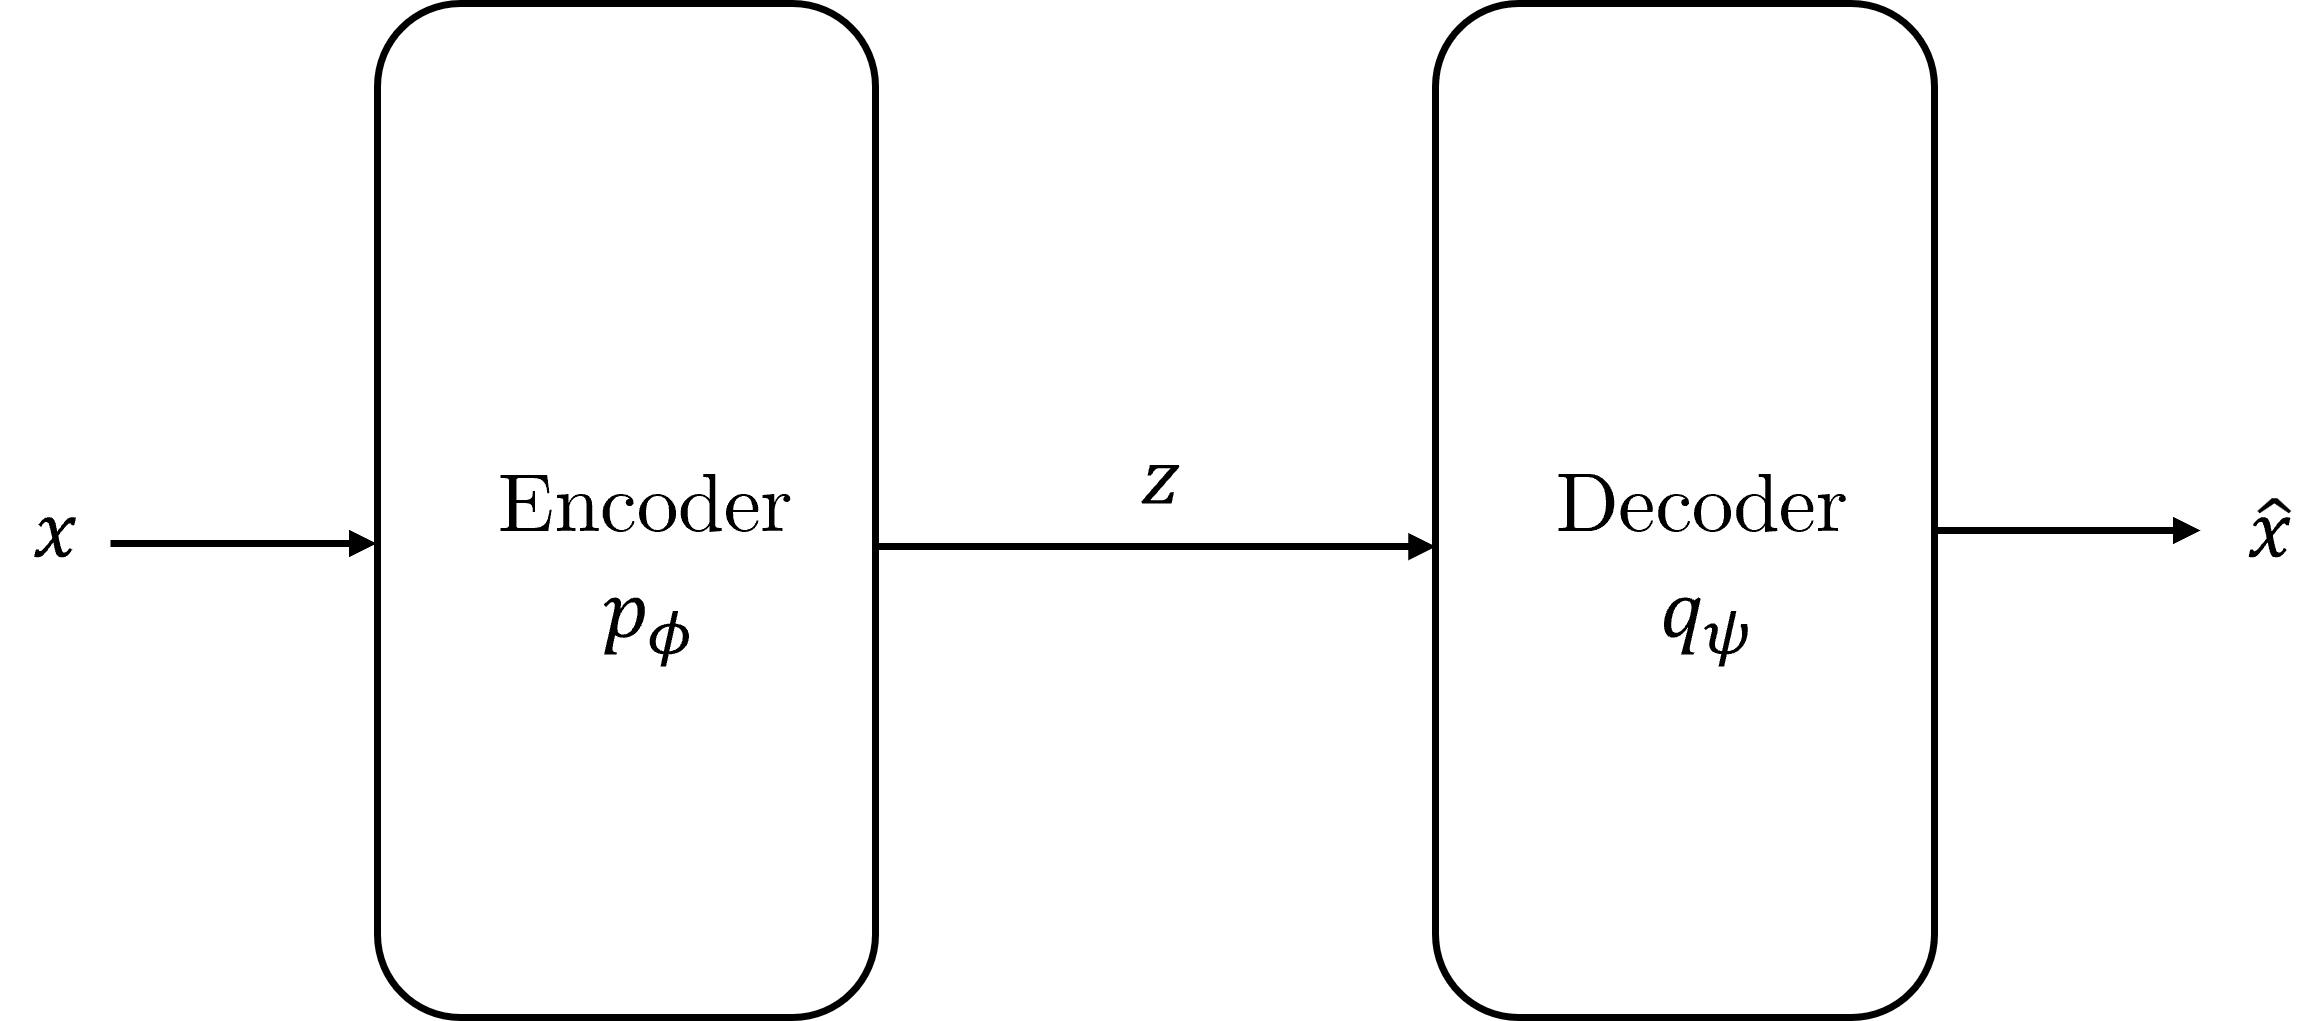
\includegraphics[width=0.5\linewidth]{figures/background/Autoencoder.png}
    \caption[Autoencoder schematics]{\textbf{schematic drawing of a Autoencoder}}
    \label{fig:Autoencoder_schematics}
\end{figure}

\subsection{Variational Autoencoders}\label{sec:VAE}

A Variational Autoencoder is similar to an Autoencoder but also with some key changes. Similar are the basic setup as a generative unsupervised learning model and the underlying encoder decoder structure. The key difference lays in the in the latent space between the encoder and decoder. Instead of having a fixed deterministic latent space VAEs operate on a probabilistic latent space~\cite{pml2Book}.
\begin{figure}
    \centering
    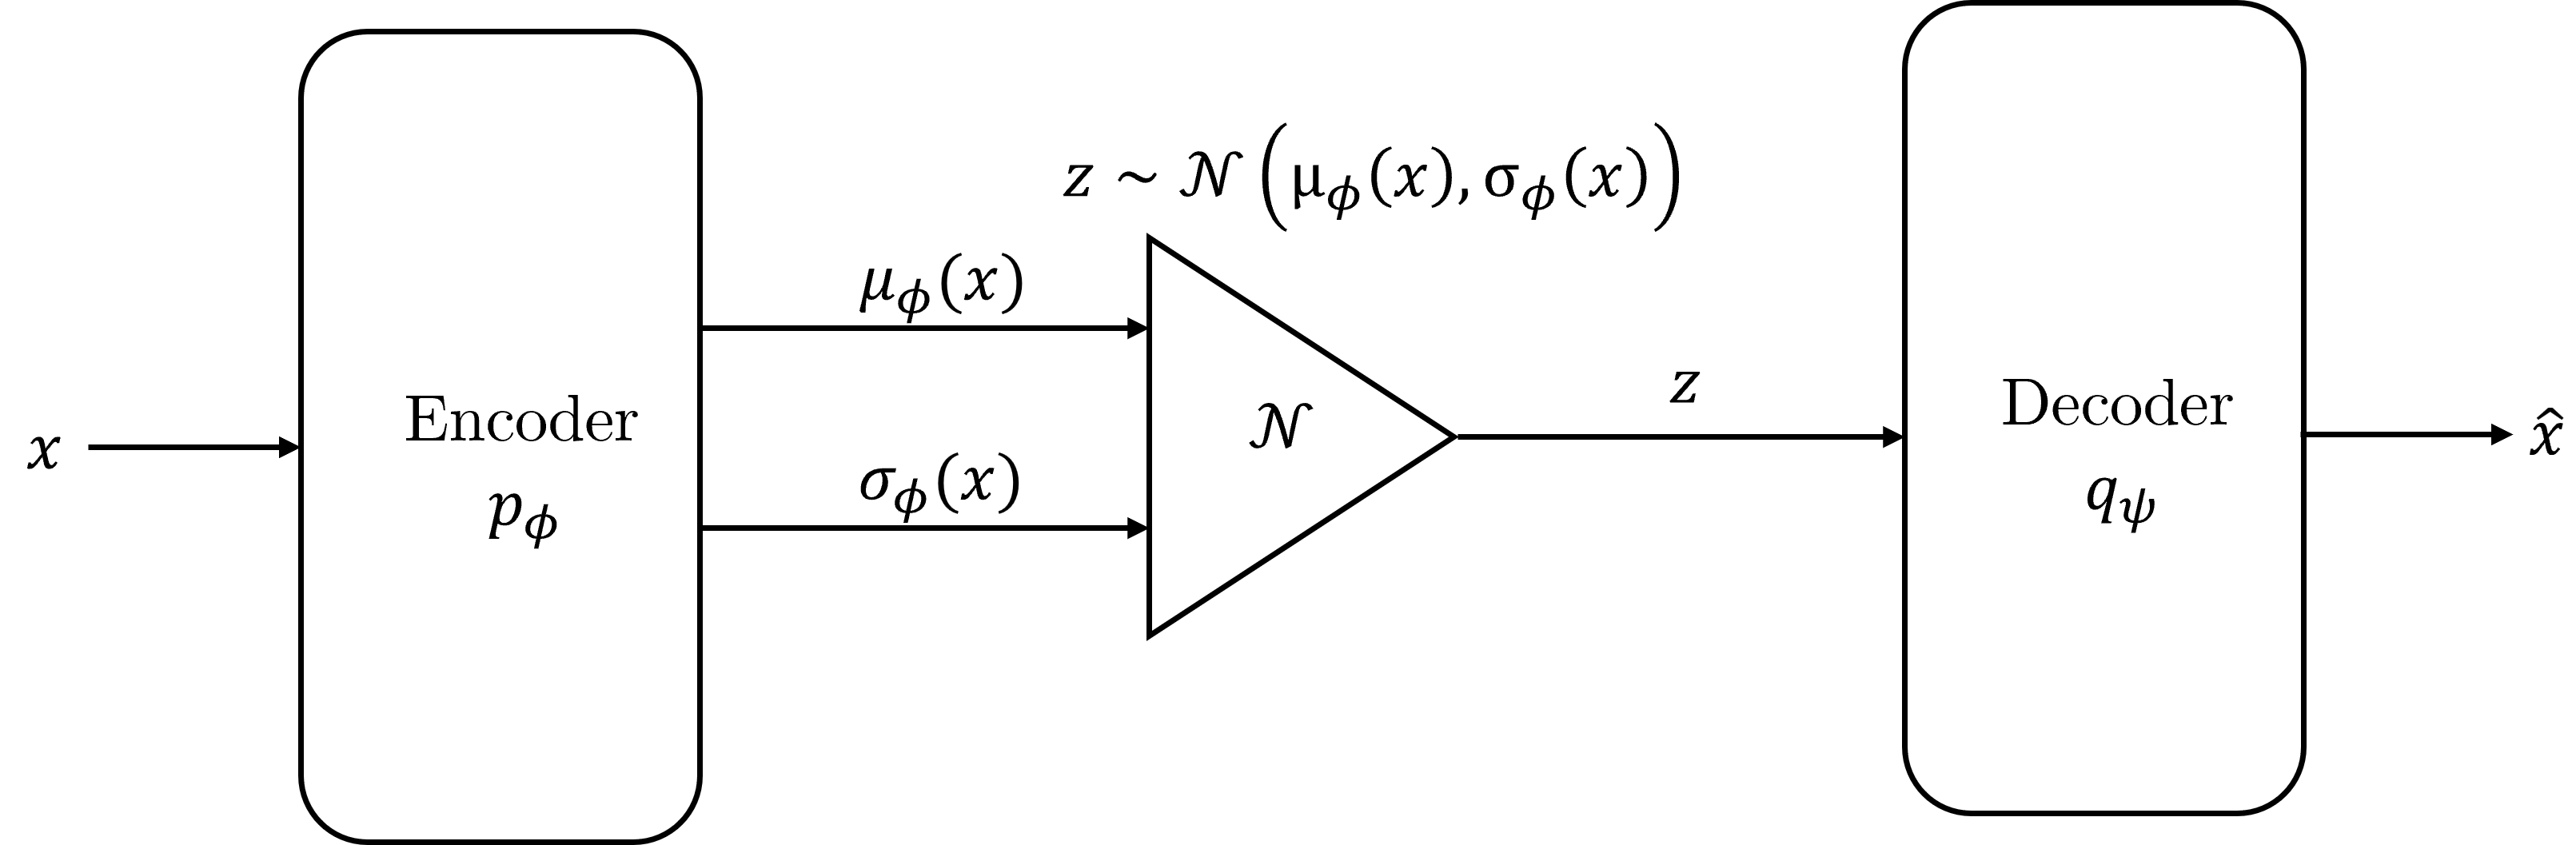
\includegraphics[width=0.7\linewidth]{figures/background/VAE.png}
    \caption[Variational Autoencoder schematics]{\textbf{schematic drawing of a Variational Autoencoder}}
    \label{fig:Variational_Autoencoder_schematics}
\end{figure}

The encoder network denoted as a approximated parameterized posterior distribution $q_\phi(z|x)$, is a conditional probability distribution in Bayesian inference with the probability of the latent variable $p(z)$ (the prior) and the evidence $p(x)$: 

\begin{align}
	q(z|x) &= \frac{p(x|z) p(z)}{p(x)} \label{eqn:Bayesian-inference}\\
	p(x) &= \int p(x|z)p(z) dz \label{eqn:p(x)}
\end{align}

In the context of a Variational Autoencoder, calculating $q(z|x)$ is not possible. As we can see in~\eqref{eqn:p(x)} accessing the evidence as the probability of the observed data is not possible because we have to integrate over all possible values of the latent variable $z$. Therefor we approximate the posterior distribution with a parameterized conditional distribution $q_\phi(z|x)$. $q_\phi(z|x)$ as known as the encoder network, parameterized with $\phi$, hereby maps input data $x$ to latent parameters like mean and variance for a gaussian distribution, of the latent distribution with random variable $z$~\cite{pml2Book}. 

On the other hand, the decoder network takes samples from the latent space with latent variables $z$ and reconstructs the data from these samples, generating a parameterized probabilistic distribution over the data given the latent variables $p_\psi(x|z)$~\cite{pml2Book}.

As mentioned before the objective in training a Variational Autoencoder is to find parameters $\phi$ and $\psi$ and matches best the true posterior distribution. In order to do so we can use the Evidence Lower Bound as the objective function. We go a bit deeper into the fundamentals of the Evidence Lower bound in \secref{sec:ELBO}. \\
During training, the VAE aims to maximize the ELBO by iteratively adjusting its parameters $\phi$ and $\psi$ using backpropagation. The encoder network maps the input data to a distribution over latent variables, while the decoder network reconstructs the data from the sampled latent variables. The reparameterization trick similar to SAC in \secref{sec:SAC} is employed to ensure differentiability during backpropagation through the stochastic sampling process~\cite{pml2Book}.


% Explain the concept of a latent variable and how it relates to VAEs
% Describe the architecture of a VAE and how it differs from a traditional autoencoder
% Explain how the encoder and decoder are trained using a variational inference approach
% Describe the role of the Kullback-Leibler (KL) divergence in the loss function

\subsection{Conditional Variational Autoencoders}

\begin{figure}
    \begin{center}
        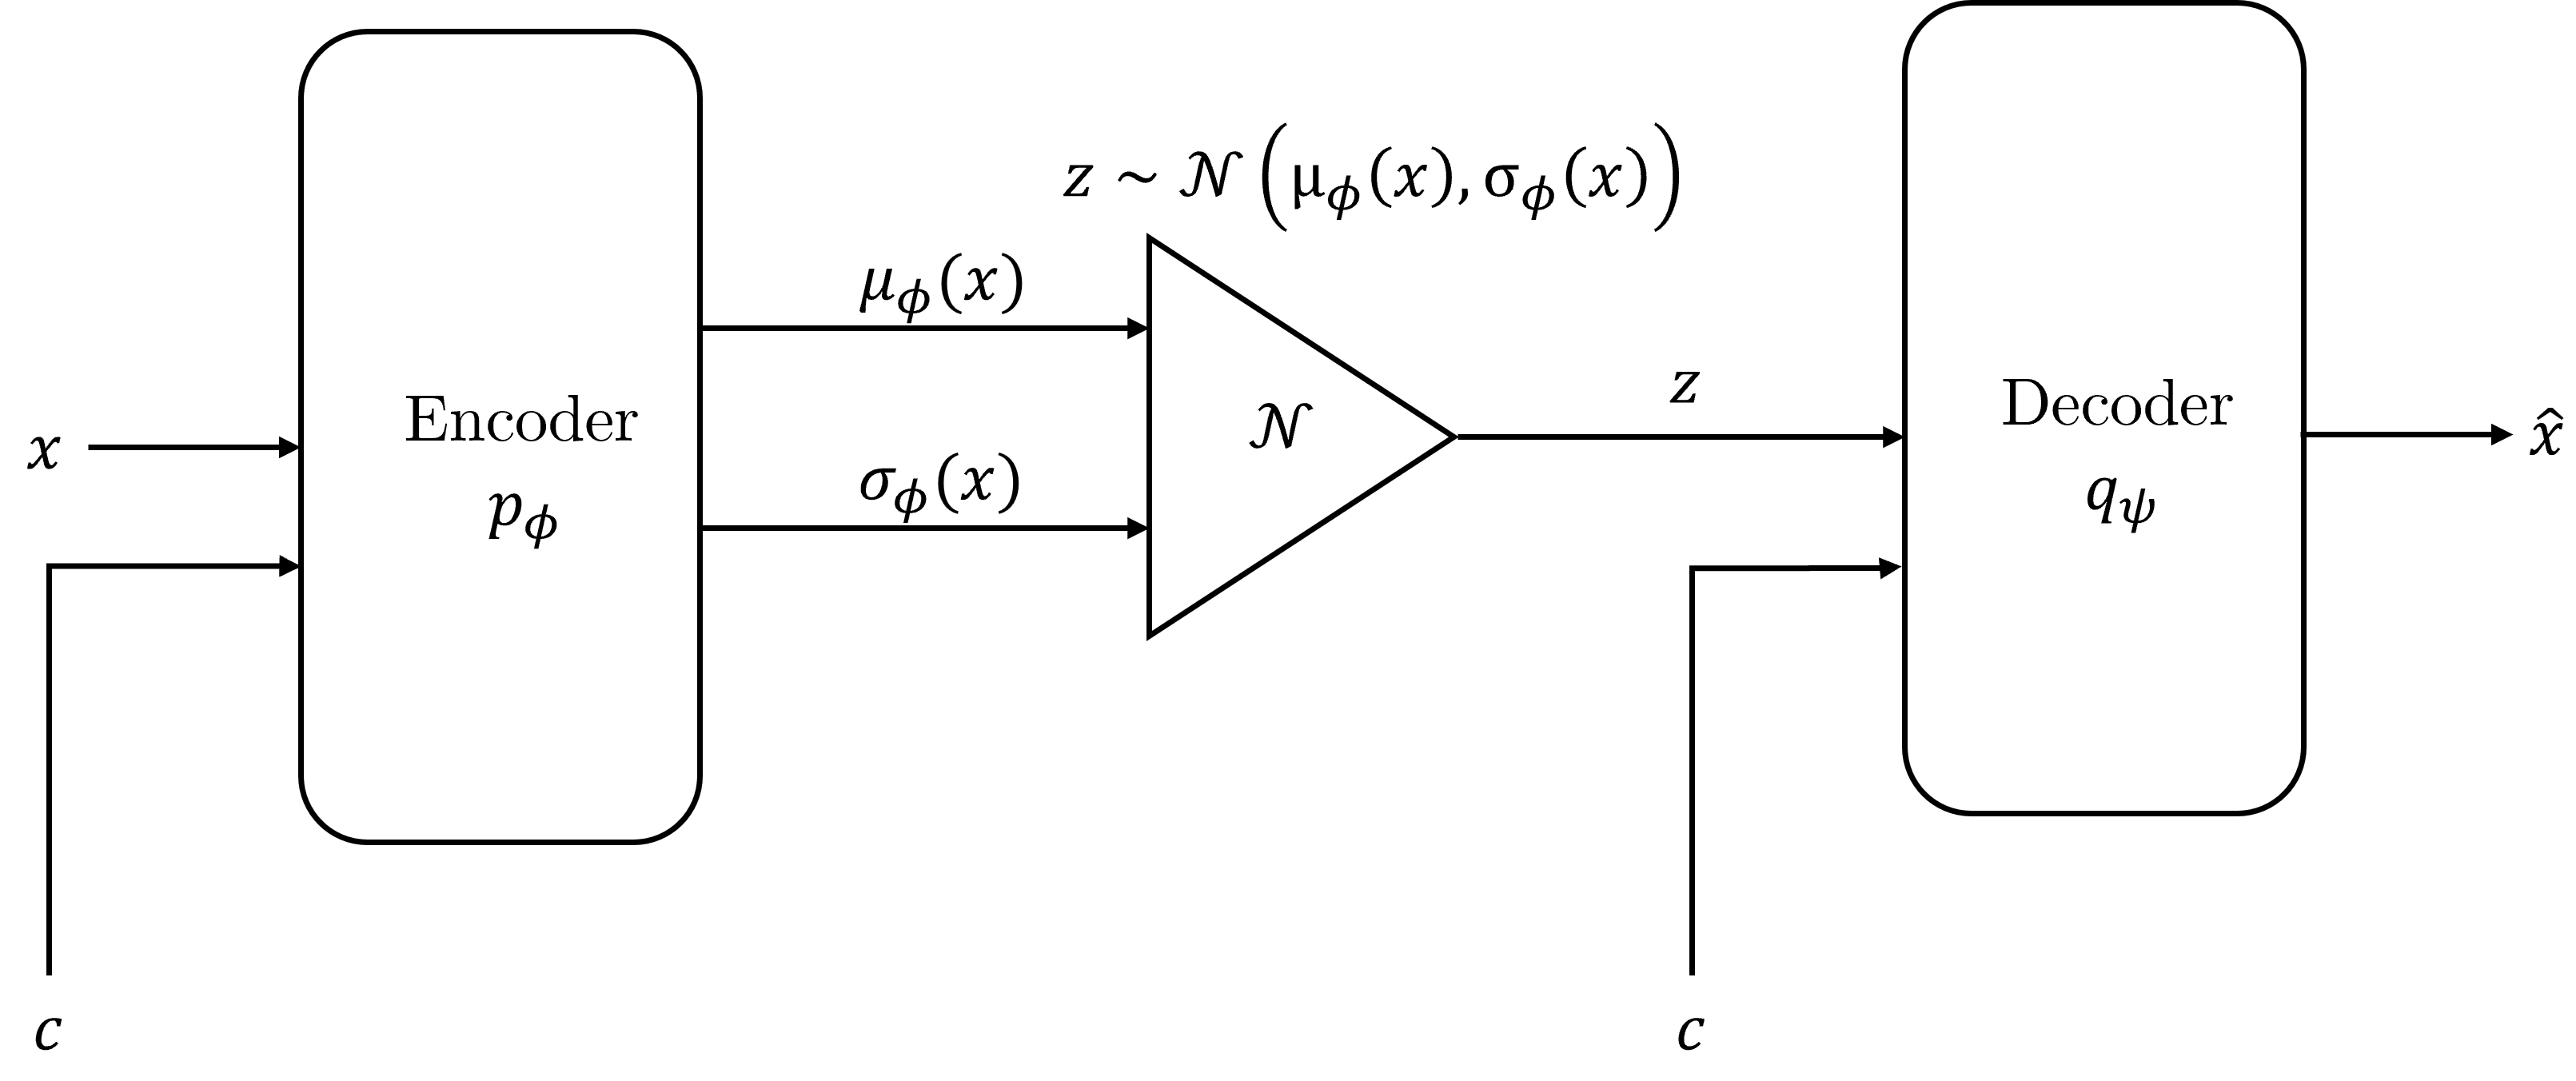
\includegraphics[width=0.7\linewidth]{figures/background/CVAE.png}
        \caption[Conditional Variational Autoencoder schematics]{\textbf{schematic drawing of a conditional Variational Autoencoder}}
        \label{fig:conditional-Variational_Autoencoder_schematics}
    \end{center}
\end{figure}
% Describe the architecture of a CVAE and how it differs from a VAE
% Explain how CVAEs can be used for supervised learning tasks
% Describe the role of the conditional input in the encoder and decoder
A Conditional Variational Autoencoder is an extension of the VAE architecture that takes into account conditional information $c$. As we can see in \figref{fig:conditional-Variational_Autoencoder_schematics} in a Conditional Variational Autoencoder, both the encoder and decoder are modified to accept an additional input that represents the conditional information~\cite{CVAE}. 

The role of the conditional input in the encoder is to help the model capture the conditional dependencies between the input data and the class label. So the conditional information could be for instance a label encoding or a set of labels that describe the class or category to which the input belongs. The encoder must learn to map both the input data and the conditional input to a meaningful latent space representation that captures the relevant information for the generation process. In the decoder, the conditional input is used to guide the generation process and ensure that the generated samples are representative of the specified class~\cite{CVAE}.

Similar to Variational Autoencoders the objective function to train the encoder and decoder is the Evidence Lower Bound. But there have to be a couple of changes to make the individual ELBO components suitable to take the conditional information $c$. The final objective can be observed in~\eqref{eqn:ELBO-CVAE}.

\subsection{Evidence Lower Bound}\label{sec:ELBO}

The Evidence Lower Bound~\cite{pml2Book} (ELBO) is a fundamental concept in the training of Variational Autoencoders (VAEs)
It is derived from the principle of variational inference and represents a lower bound on the log-likelihood of the data given the models parameters. Maximizing the ELBO is equivalent to minimizing the Kullback-Leibler (KL) divergence~\cite{pml2Book} between the true posterior distribution $q(z|x)$ over latent variables $z$ and the approximated posterior distribution $q_\phi(z|x)$ used in the VAE.

\begin{equation}\label{eqn:ELBO}
	\mathcal{L}_\text{ELBO}(x, z) = \mathbb{E}_{z\sim q_\phi(\cdot|x)} \left[ \log p_\psi(x|z) \right] - \text{KL}\left( q_\phi(z|x) \| p(z) \right)
\end{equation}

Further I will discuss the individual components of the Evidence lower bound 
\begin{itemize}
	\item \textbf{Posterior Distribution}: In general the posterior distribution $q(z|x)$ is considered as the probability of the latent variable $z$ given the observed data $x$. Specific for Variational Autoencoder it can be computed from Bayesian Inference as in~\eqref{eqn:Bayesian-inference} which is as mentioned in \secref{sec:VAE} not feasible is therefor approximated.
	\item \textbf{Likelihood}: The likelihood function $p(x|z)$ or conditional likelihood in the context of probabilistic models is the probability distribution of the observed data $x$ given the latent variables $z$. Dependent on the observed data it is possible to chose from a set of different probability distributions. Examples are a multivariate gaussian distribution for continuous data, a Bernoulli distribution for binary data or categorical distribution for discrete data with multiple categories.
	\item \textbf{Prior Distribution}: The prior distribution $p(z)$ is a probabilistic distribution that represents the initial belief or assumption about the latent variables $z$ in Bayesian inference. Additional $p(z)$ serves in Variational Autoencoder as a regularizer during training as it encourages the VAE to learn meaningful and smooth latent representations in the latent space. Most popular choice for the prior distribution is the standard normal distribution $\mathcal{N}(0, I)$.  
	\item \textbf{Evidence}: p(x) represents the evidence, also known as the marginal likelihood or model evidence, in the context of Bayesian statistics. It is the probability of the observed data $x$ given a particular statistical model. The evidence serves in~\eqref{eqn:p(x)} as a normalization constant, ensuring that the posterior distribution $q(z|x)$ over model parameters integrates to 1. It quantifies how well the model, with its specific set of parameters, explains or fits the observed data.
	\item \textbf{Reconstruction Loss}: 
	\begin{equation}\label{eqn:general-reconstruction-loss}
		\mathbb{E}_{z\sim q(\cdot|x)} \left[ \log p(x|z) \right] \approx \mathbb{E}_{z\sim q_\phi(\cdot|x)} \left[ \log p_\psi(x|z) \right]
	\end{equation}
	Therm (\ref{eqn:general-reconstruction-loss}) measures the similarity between the reconstructed data and the original input. 
	Described in words it is the expected log-likelihood of the data given the latent variables, which is computed by sampling from the approximating distribution $q_\phi(z|x)$ and evaluating the likelihood $p_\psi(x|z)$ using the decoder network.
	\item \textbf{KL Divergence Loss}: 
	\begin{equation}
		\text{KL}\left( q(z|x) \| p(z) \right) \approx \text{KL}\left( q_\phi(z|x) \| p(z) \right)
	\end{equation}
	This term quantifies the difference between the approximated parameterized posterior distribution $q_\psi(z|x) $ over latent variables $z$ and a chosen prior distribution $p(z)$. As mentioned before it is a popular choice to use a standard normal distribution $p(z)=\mathcal(N)(0,I)$ as the prior distribution. The KL divergence encourages the latent variables to be close to the prior distribution, promoting regularization and preventing overfitting.
\end{itemize}

\todo{Explain prior and posterior distributions}
\iffalse
The posterior distribution, denoted as q(z|x), is a conditional probability distribution in Bayesian inference. In the context of Variational Autoencoders (VAEs), the posterior distribution refers to the distribution of the latent variables z given the observed data x.
In VAEs, the encoder network parameterizes the approximate posterior distribution q(z|x), which takes the input data x as input and outputs the parameters (e.g., mean and variance) of the distribution over the latent variables z. The encoder learns to map the data x to a distribution in the latent space, where each point in the latent space represents a potential encoding of the data.
The posterior distribution q(z|x) is essential in the VAE framework because it allows the model to learn meaningful and compressed representations of the input data. By optimizing the ELBO (Evidence Lower Bound), VAEs simultaneously maximize the likelihood term (the data reconstruction term) and minimize the KL divergence term, encouraging the approximate posterior to be close to the prior distribution p(z).
The posterior distribution q(z|x) plays a central role in VAEs, enabling the model to capture the underlying structure of the data and support various applications, such as data generation and latent space interpolation.

The prior distribution, denoted as p(z), is a probabilistic distribution that represents our initial belief or assumption about the latent variables z in Bayesian inference. In the context of Variational Autoencoders (VAEs), the prior distribution refers to the distribution of the latent variables z before observing any data.
In VAEs, the prior distribution is typically chosen to be a simple and well-known distribution, such as a standard normal distribution with zero mean and unit variance, i.e., p(z) = N(0, 1). Using a standard normal distribution as the prior is a common choice due to its simplicity and ease of sampling.
The prior distribution serves as a regularizer during training and plays a crucial role in VAEs' generative process. By incorporating the prior distribution in the ELBO (Evidence Lower Bound) objective function, VAEs are encouraged to learn meaningful and smooth latent representations. The KL divergence term in the ELBO measures the difference between the approximate posterior distribution q(z|x) (learned by the encoder) and the prior distribution p(z). Minimizing this term ensures that the approximate posterior is close to the prior distribution, promoting regularization and preventing overfitting.
The choice of the prior distribution can impact the VAEs performance and the characteristics of the generated data. While a standard normal distribution is commonly used, VAEs can be adapted to use other types of priors, such as uniform distributions or more complex distributions, depending on the specific requirements of the application.
\fi

The basic notation of the Evidence Lower Bound for Variational Autoencoders as in~\eqref{eqn:ELBO} can be easily extented for an Conditional Variational Autoencoder:
\begin{equation}\label{eqn:ELBO-CVAE}
	\mathcal{L}_\text{ELBO}(x, z, c) = \mathbb{E}_{z\sim q_\phi(\cdot|x, c)} \left[ \log p_\psi(x|z, c) \right] - \text{KL}\left( q_\phi(z|x, c) \| p(z|c) \right)
\end{equation}
\todo{Describe also the components of the CVAE ELBO }

By optimizing the ELBO, VAEs effectively learn to approximate the true posterior distribution and generate meaningful latent representations of the data, enabling various tasks such as data generation, interpolation, and denoising within a Bayesian framework~\cite{pml2Book}.

\subsection{VAEs and CVAEs in Practice}

% Provide examples of real-world applications of VAEs and CVAEs, such as image and text generation, and conditional image generation
% Explain how VAEs and CVAEs can be used for data compression and denoising
% Describe the advantages and limitations of VAEs and CVAEs compared to other % generative models

VAEs and CVAEs have been successfully applied to a wide range of real-world applications. In image generation~\cite{pml2Book}, VAEs have been used to generate novel images of faces, objects, and scenes~\cite{pml2Book}. Similarly, CVAEs have been used for conditional image generation, allowing for the generation of images based on specific attributes or classes. In text generation, VAEs have been used to generate natural language sentences and paragraphs.

VAEs and CVAEs can also be used for data compression~\cite{VAE_Compression} and denoising~\cite{VAE_denoising}. By learning a compressed representation of the input data, VAEs and CVAEs can reduce the dimensionality of the input space while preserving important features. Similarly, by learning to reconstruct the original input from noisy or corrupted data, VAEs and CVAEs can be used for denoising and data restoration.

One of the advantages of VAEs and CVAEs is their ability to learn a continuous latent representation of the input data. This allows for easy manipulation and exploration of the latent space, enabling applications such as image editing and style transfer~\cite{VAE}.

However, VAEs and CVAEs have some limitations. The generated samples may not be as sharp or detailed as those produced by other generative models such as GANs~\cite{VAEvsGAN}. Additionally, the trade-off between the reconstruction loss and the KL divergence term can be difficult to balance, potentially leading to overfitting or underfitting~\cite{KL_Loss_R_Loss}. Nonetheless, VAEs and CVAEs remain a popular and powerful tool for generative modeling and data compression.


% \subsection{Extensions to VAEs and CVAEs}
% 
% Describe extensions to the basic VAE and CVAE architectures, such as hierarchical VAEs and semi- supervised VAEs
% Explain how VAEs and CVAEs can be combined with other models, such as Generative Adversarial % Networks (GANs)

% \subsection{Current and Future Directions}
% 
% Describe current research trends in VAEs and CVAEs, such as improving the quality of generated samples and addressing the mode collapse problem
% Discuss potential future applications of VAEs and CVAEs, such as in healthcare and climate modeling
% Explain challenges that must be addressed in order for VAEs and CVAEs to continue to advance

% \subsection{Conclusion}
% 
% Summarize the main points of the chapter
% Emphasize the importance of VAEs and CVAEs in a variety of fields
% Encourage further exploration of the topic.

\section{Kinematics}

Kinematics is the study of motion, specifically the description and analysis of the position, velocity, and acceleration of objects or systems~\cite{ForwardKinematics}~\cite{CCD} without considering the forces causing the motion. It focuses on understanding the spatial relationships and geometrical aspects of moving objects. The following sections provide an insight into forward and inverse kinematics for kinematic chains. Those two concepts are often used in robotics, animation, virtual reality or even protein folding. 

\subsection{Forward kinematics}

Forward kinematics is a concept from robotics that involves determining the position and orientation of an end-effector, like a gripper of a robot arm, based on the joint angles and geometric parameters, like segment length, of the system. It provides a mathematical model for mapping the joint angles to the end-effector position in order to understand the overall configuration and motion of the robot.~\eqref{alg:FK} describes a forward kinematics implementation. 
% \begin{algorithm}
    \caption{Forward Kinematics}\label{alg:FK}
    \begin{algorithmic}
        \State{} Input: Current joint angles $q$, Segment Length $l$.
        \State{} Define origin position in 2D space: $p \leftarrow (0, 0)$
        \For{each $i$ in $[0, \ldots, N - 1]$}
            \State{} Update position
            \State{} $p_0 \leftarrow p_0 + \cos(q_i) * l_i$
            \State{} $p_1 \leftarrow p_1 + \sin(q_i) * l_i$
        \EndFor{}
\end{algorithmic}
\end{algorithm}

\begin{algorithm}
    \caption{Forward Kinematics}\label{alg:FK}
    \begin{algorithmic}
        \State{} Input: Current joint angles $q$, Segment Length $l$.
        \State{} Define origin position in 2D space: $p \leftarrow (0, 0)$
        \For{each $i$ in $[0, \ldots, N - 1]$}
            \State{} Update position
            \State{} $p_0 \leftarrow p_0 + \cos(q_i) * l_i$
            \State{} $p_1 \leftarrow p_1 + \sin(q_i) * l_i$
        \EndFor{}
\end{algorithmic}
\end{algorithm}

Throughout this thesis this function is used with a constant segment length $l = \{1\}^N$ therefor it is referred to as in~\eqref{eqn:FK} which maps an angle configuration $q$ into the end-effector position in 2D space.

\begin{equation}\label{eqn:FK}
	FK: \mathbb{R}^N \to \mathbb{R}^2
\end{equation}

\subsection{Inverse kinematics}

Inverse kinematics (IK) is a fundamental problem in robotics, animation or virtual reality that involves finding a required joint angle configuration or positions to reach a desired end-effector position and optionally a desired orientation~\cite{InverseKinemaitcs}. It plays a crucial role in controlling the motion and manipulation of robotic systems, enabling them to interact with the environment and perform complex tasks. 
In this section you will find a brief summary of existing approaches, a deeper explanation of the Cyclic Coordinate Descent algorithm and the description of the used inverse kinematics RL environment.

\subsubsection{Existing Approaches to Solve Inverse Kinematics}

Numerous approaches have been proposed to solve the inverse kinematics problem. These approaches can be broadly categorized into: 
\begin{itemize}
	\item analytical methods~\cite{IK_ClosedForm}: rely on geometric methods to derive closed form solutions.
	\item numerical methods~\cite{NumericalMethods}: iteratively approximate the joint angles that satisfy the desired end-effector position and orientation.
	\item heuristic methods~\cite{NumericalMethods}: iteratively propagate positions along the kinematic chain to converge on the desired end-effector position.
	\item sampling-based methods~\cite{NumericalMethods}: randomized search strategy to explore the joint space and find feasible solutions to the inverse kinematics problem
\end{itemize}

% \subsubsection{Existing Approaches to Solve Inverse Kinematics Extended}

% \textbf{Analytical Methods}: Some robotic systems with simple geometries and kinematic structures can be solved analytically using closed-form solutions. Analytical methods often rely on geometric techniques and mathematical equations such as the Denavit-Hartenberg (DH) parameters to derive explicit formulas for the joint angles. These methods provide fast and exact solutions when applicable, but they are limited to specific cases with well-defined geometric relationships.

% \textbf{Numerical Methods}: Numerical methods for inverse kinematics aim to iteratively approximate the joint angles that satisfy the desired end-effector position and orientation. Jacobian-based methods, such as the Jacobian transpose method and the Jacobian pseudo-inverse method, leverage the Jacobian matrix to relate the end-effector velocities to the joint velocities. These methods iteratively adjust the joint angles based on the discrepancy between the actual and desired end-effector positions. Other numerical techniques, including cyclic coordinate descent, Gauss-Newton, Levenberg-Marquardt, and optimization algorithms like Particle Swarm Optimization and Genetic Algorithms, aim to find optimal joint configurations by minimizing an objective function that represents the error between the desired and actual end-effector positions.

% \textbf{Heuristic Methods}: Heuristic methods, such as the Forward and Backward Reaching Inverse Kinematics (FABRIK) algorithm, iteratively propagate positions along the kinematic chain to converge on the desired end-effector position. These methods provide an intuitive and efficient way to solve inverse kinematics problems and handle complex robotic structures with multiple degrees of freedom.

% \textbf{Sampling-Based Methods}: Sampling-based methods, such as Randomized Kinodynamic Planning (RRT), adopt a randomized search strategy to explore the joint space and find feasible solutions to the inverse kinematics problem. By sampling and connecting valid configurations in the joint space, these methods can discover feasible joint angles that satisfy the end-effector constraints.

% \textbf{Machine Learning-based Methods}: Machine learning approaches, including neural networks and reinforcement learning algorithms, have been increasingly explored for solving inverse kinematics. Neural networks can be trained to approximate the inverse kinematics mapping based on input-output data pairs. Reinforcement learning algorithms, such as Soft Actor-Critic (SAC), can learn inverse kinematics policies through trial-and-error interactions with the environment, optimizing joint configurations to achieve desired end-effector positions.

\subsubsection{Cyclic Coordinate Descent}

Cyclic Coordinate Descent (CCD)~\cite{NumericalMethods} is a popular numerical method for solving inverse kinematics. It is an iterative algorithm that adjusts the joint angles of a robotic system one at a time, from a base joint to the end-effector, in order to align the end-effector with the desired target position.

\begin{algorithm}
    \caption{Cyclic Coordinate Descent Pseudo Code}\label{alg:CCD}
    \begin{algorithmic}
        \State{} Input: Current joint angles $q$, Desired end-effector position $p_\text{target}$.
        \While{unitl convergence}
            \For{each $i$ in $[N-1, \ldots, 0]$}
                \State{} Calculate vector from current joint position to end-effector position:
                \State{} $v_\text{current} \leftarrow p_{N-1} - p_i$

                \State{} Calculate vector from current joint position to target position:
                \State{} $v_\text{target} \leftarrow p_\text{target} - p_i$

                \State{} Calculate the necessary rotation to align $v_\text{current}$ with $v_\text{target}$:
                \State{} $\delta q_i \leftarrow \text{angle\textunderscore between}(v_\text{current}, v_\text{target})$

                \State{} Update joint angle:
                \State{} $q_i \leftarrow q_i + \delta q_i$
            \EndFor{}
        \EndWhile{}
\end{algorithmic}
\end{algorithm}

The algorithm works by iteratively updating the joint angles based on the discrepancy between the current and desired end-effector positions ($p_\text{target}$). At each iteration, CCD focuses on a single joint and adjusts its angle to minimize the positional error. By sequentially updating the joint angles in a cyclic manner, CCD aims to converge towards a solution that satisfies the desired end-effector position.

As illustrated in \algoref{alg:CCD} and \figref{fig:background/CCD geometry} in each iteration, CCD calculates the vector from the current joint position $p_i$ with $p_i$ as the position of the $i$th joint with $i \in \{0, \ldots, N-1\}$, to the end-effector position ($v_\text{current}$) and the vector from the current joint position to the target position ($v_\text{target}$). By finding the rotation necessary to align $v_\text{current}$ with $v_\text{target}$, represented as $\delta q_i$, the algorithm updates the joint angle accordingly. This process is repeated for each joint in the kinematic chain until convergence is achieved.
\begin{figure}
	\centering
	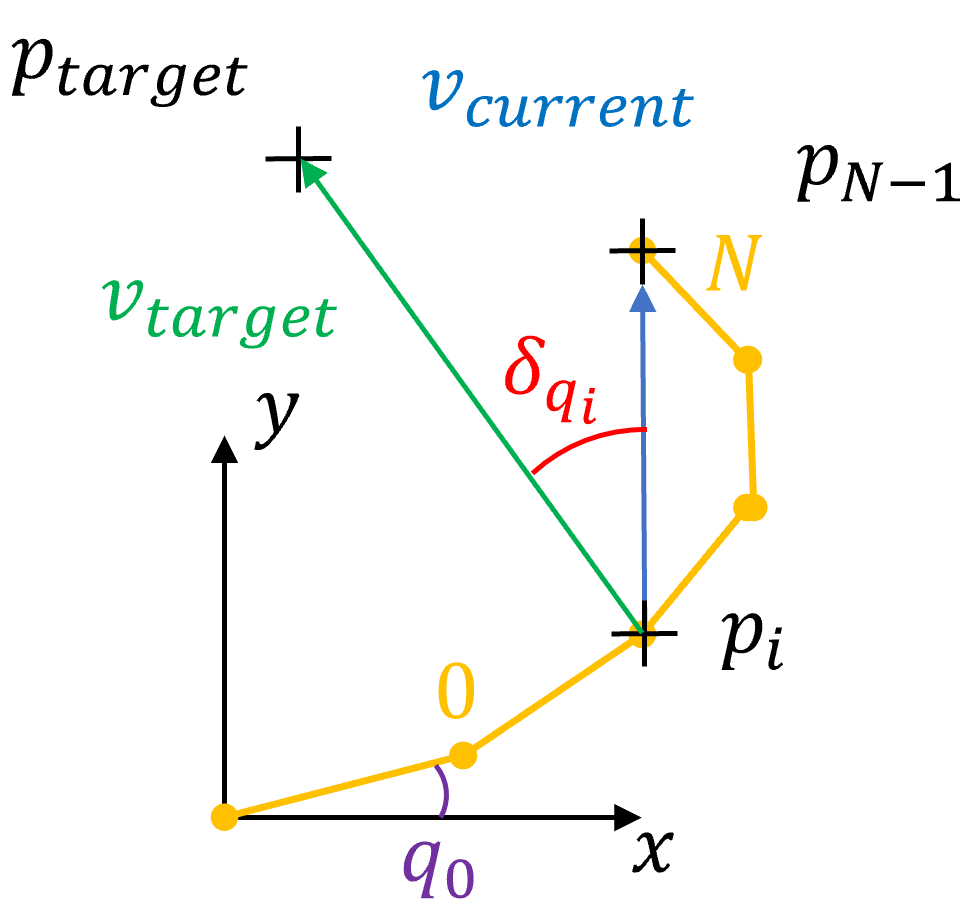
\includegraphics[width=0.4\textwidth,]{figures/background/CCD_geometry.png}
	\caption[CCD geometry]{CCD geometry: Shown is the geometry of one step in \algoref{alg:CCD}. $p_\text{target}$ is the target position. $p_i$ is the 2D position of each joint. Not that we start with the first joint outside the origin since the base position is fixed to the origin.}
	\label{fig:background/CCD geometry}
\end{figure}

This afore mentioned strategy can be reviewed in \figref{fig:ccd_trajectory}. Here we can see that the strategy appears to move closer and closer to the origin before heading towards the target position in blue.
\begin{figure}
    \begin{center}
        \subfloat[$N = 2$ with 5 iterations]{
            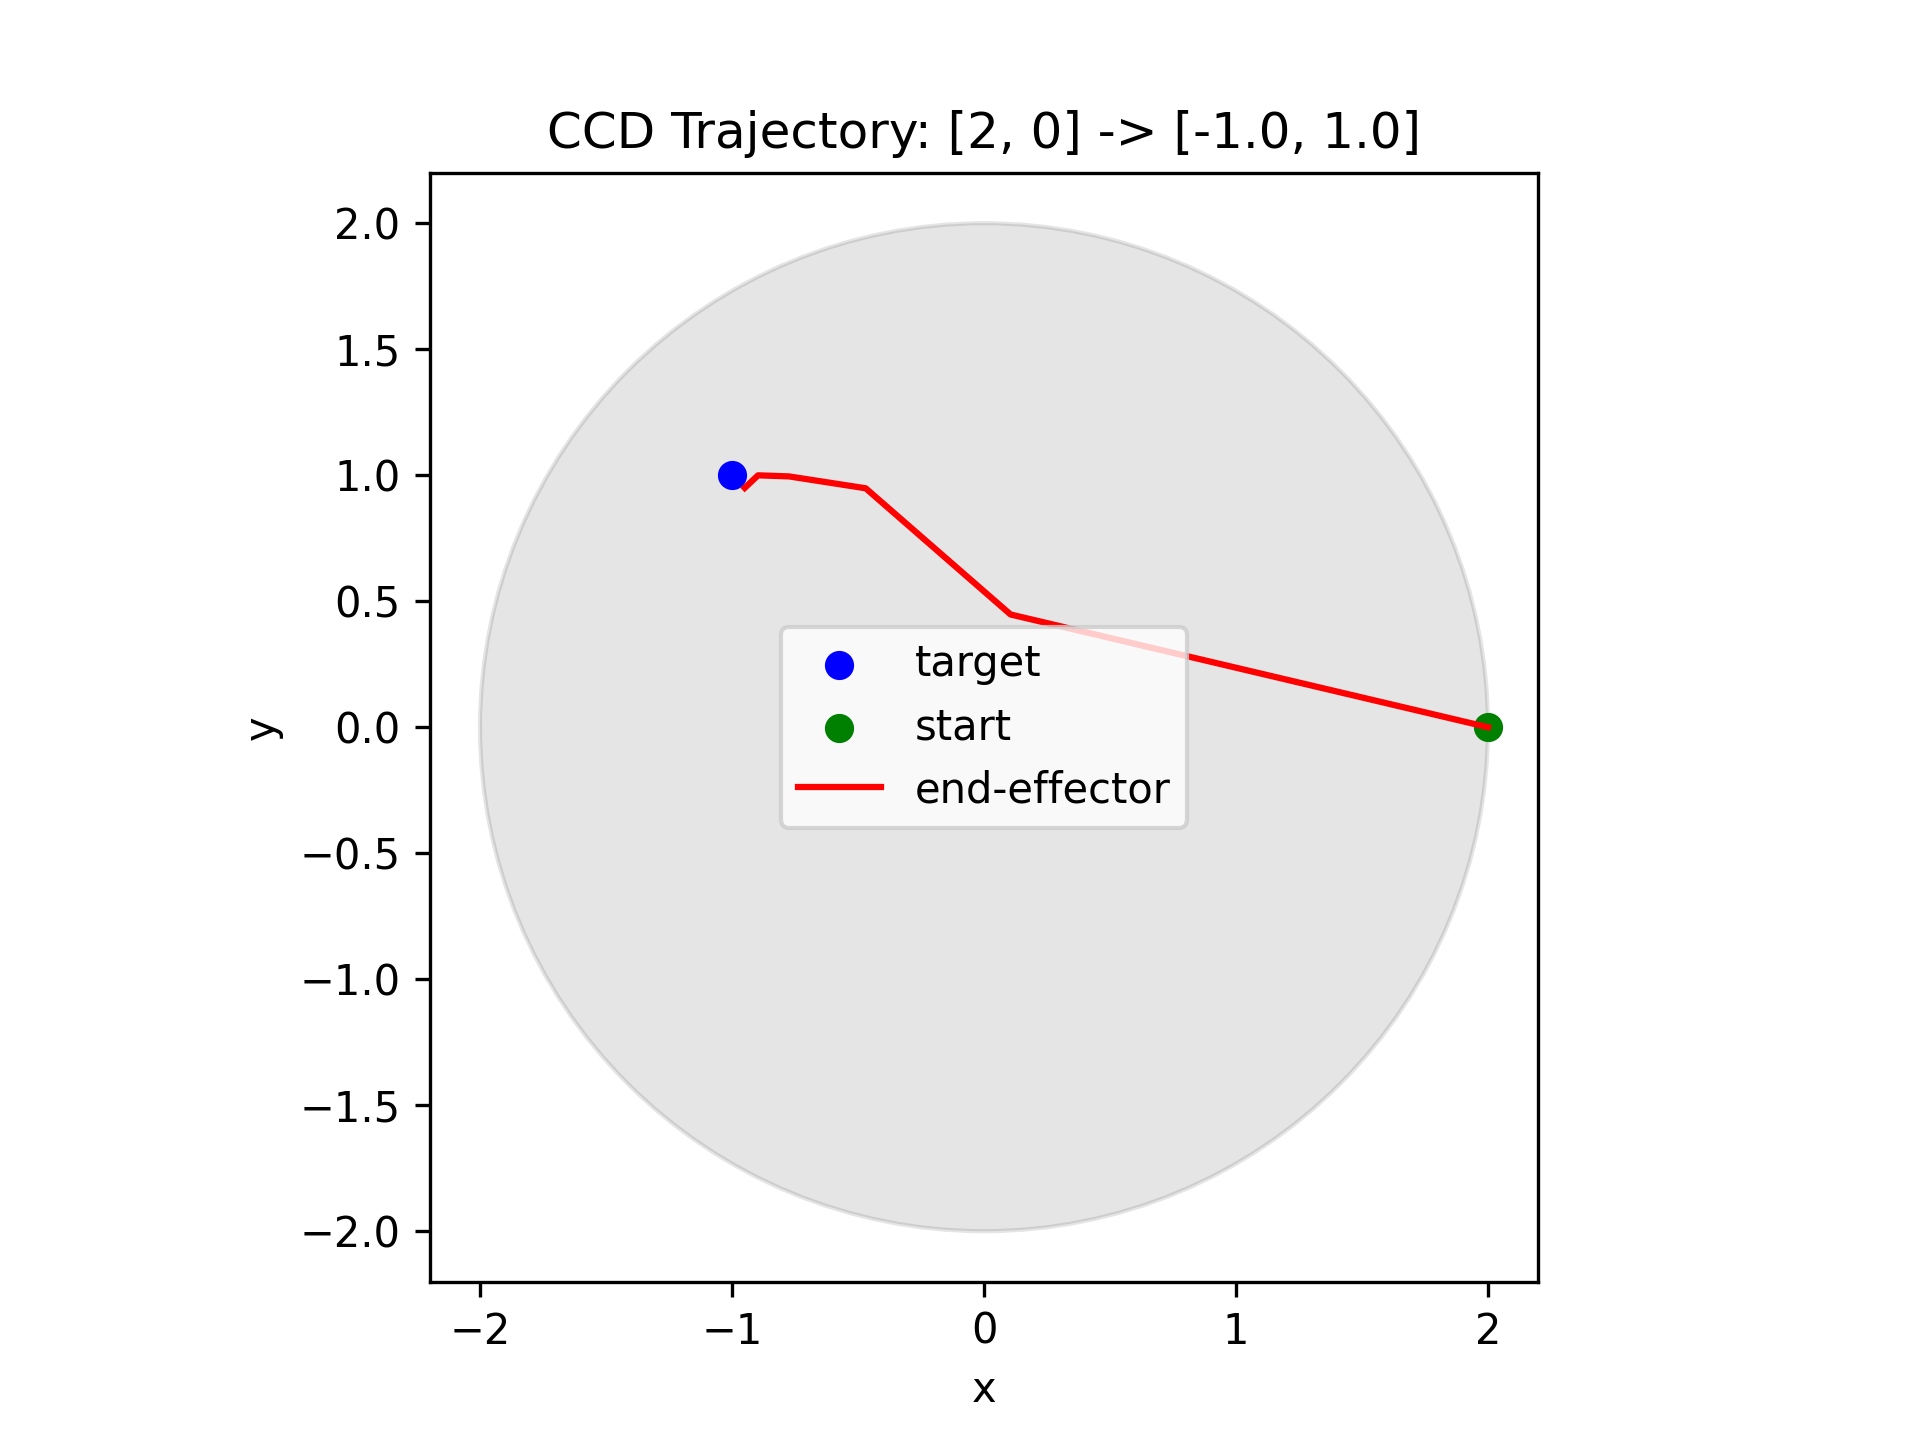
\includegraphics[width=0.31\linewidth]{figures/background/CCD_trajectory_2.png}
            \label{fig:ccd_trajectory/2}
            }
        \hfill
        \subfloat[$N = 5$ with 11 iterations]{
            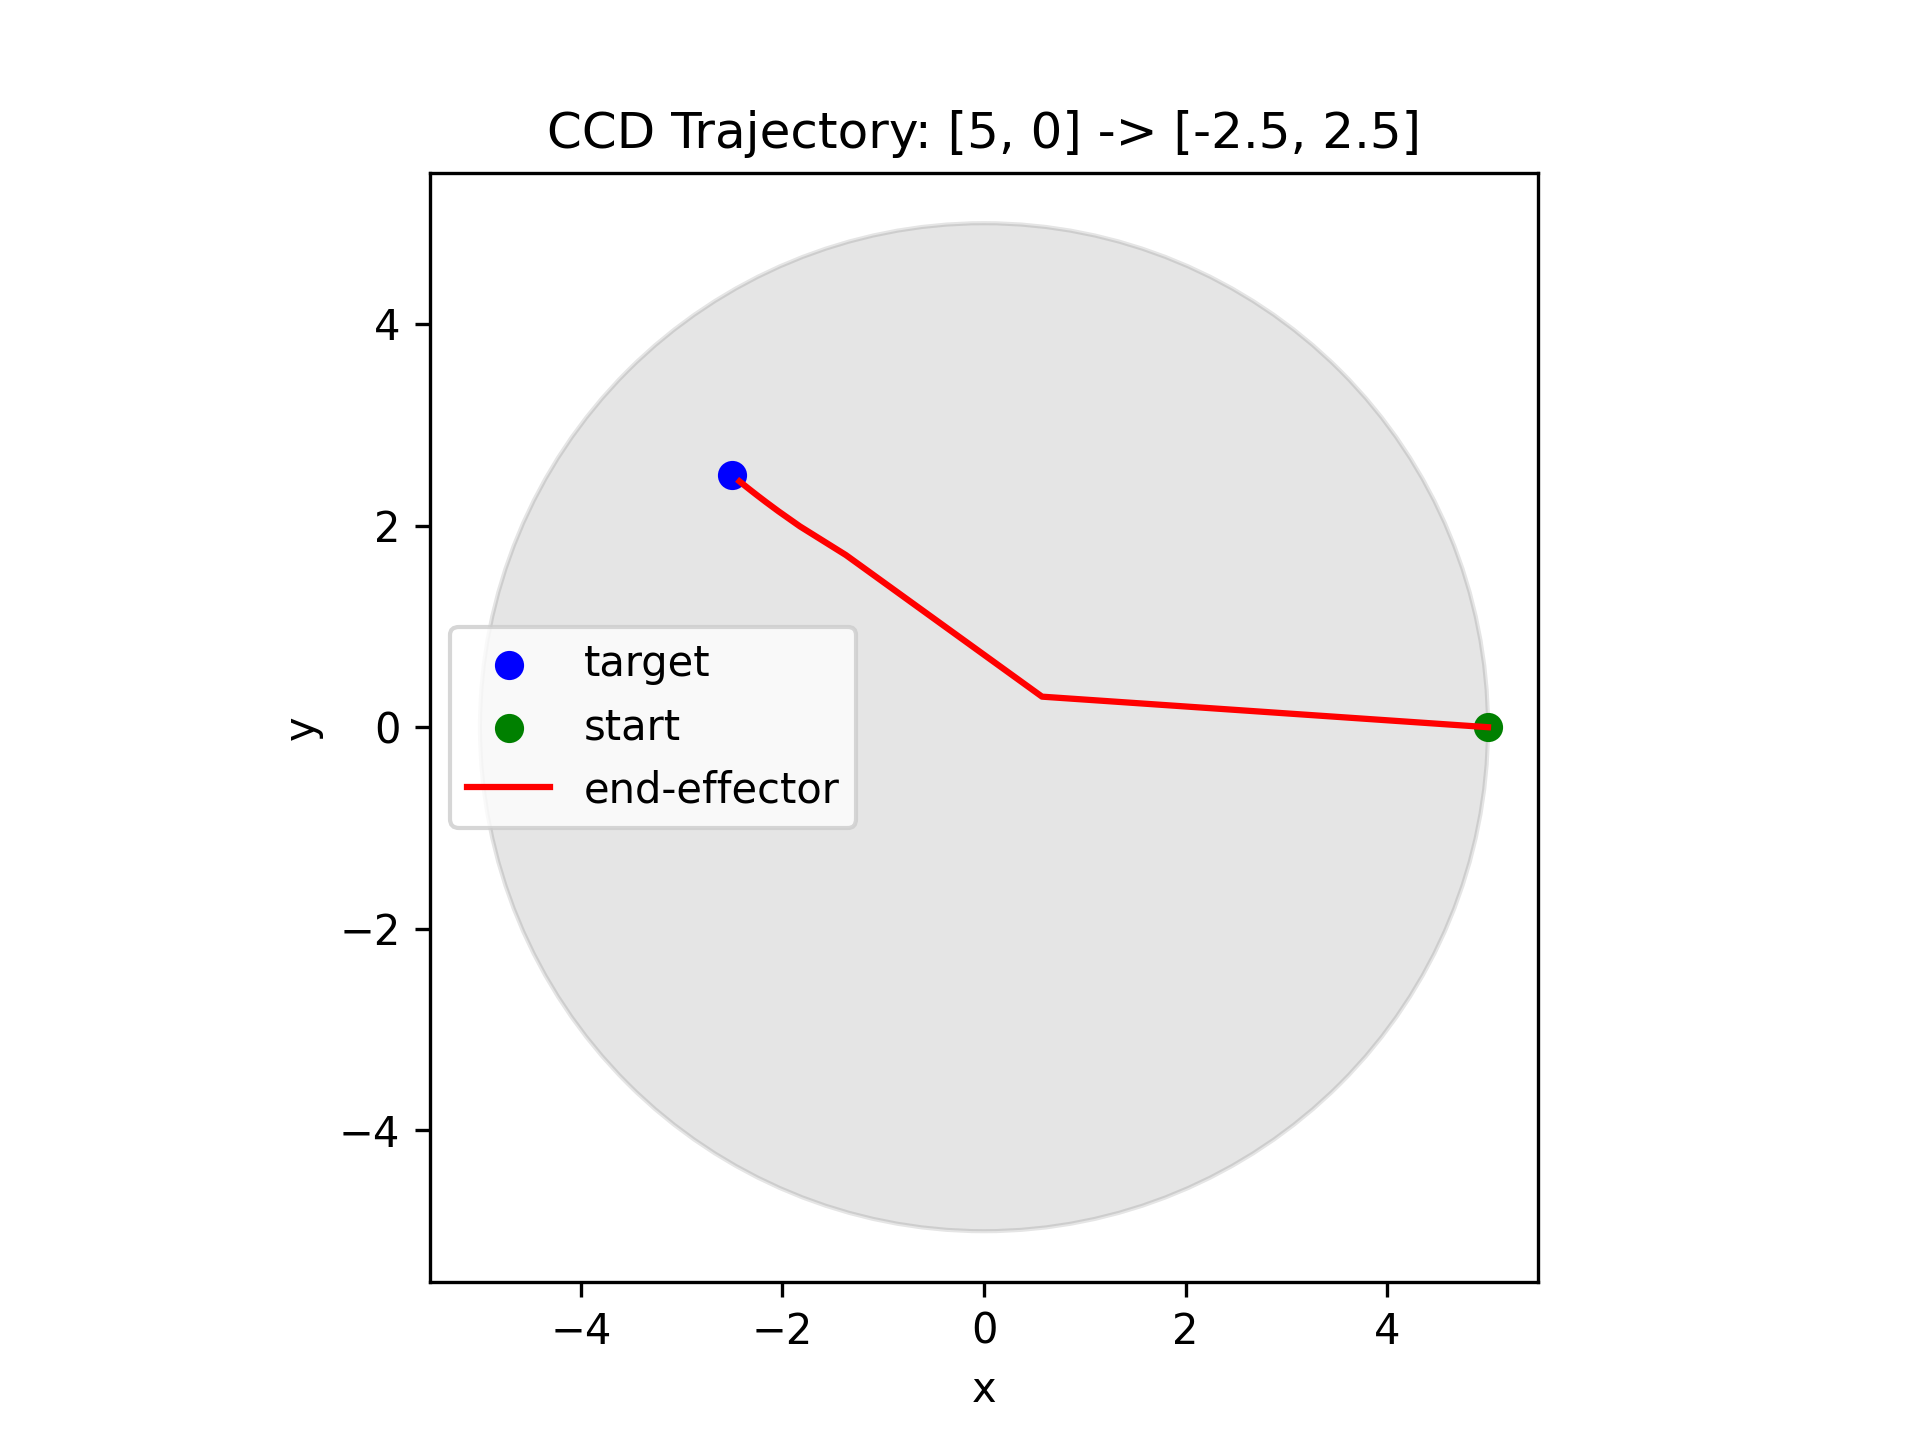
\includegraphics[width=0.31\linewidth]{figures/background/CCD_trajectory_5.png}
            \label{fig:ccd_trajectory/5}
            } 
		\hfill
        \subfloat[$N = 10$ with 64 iterations]{
            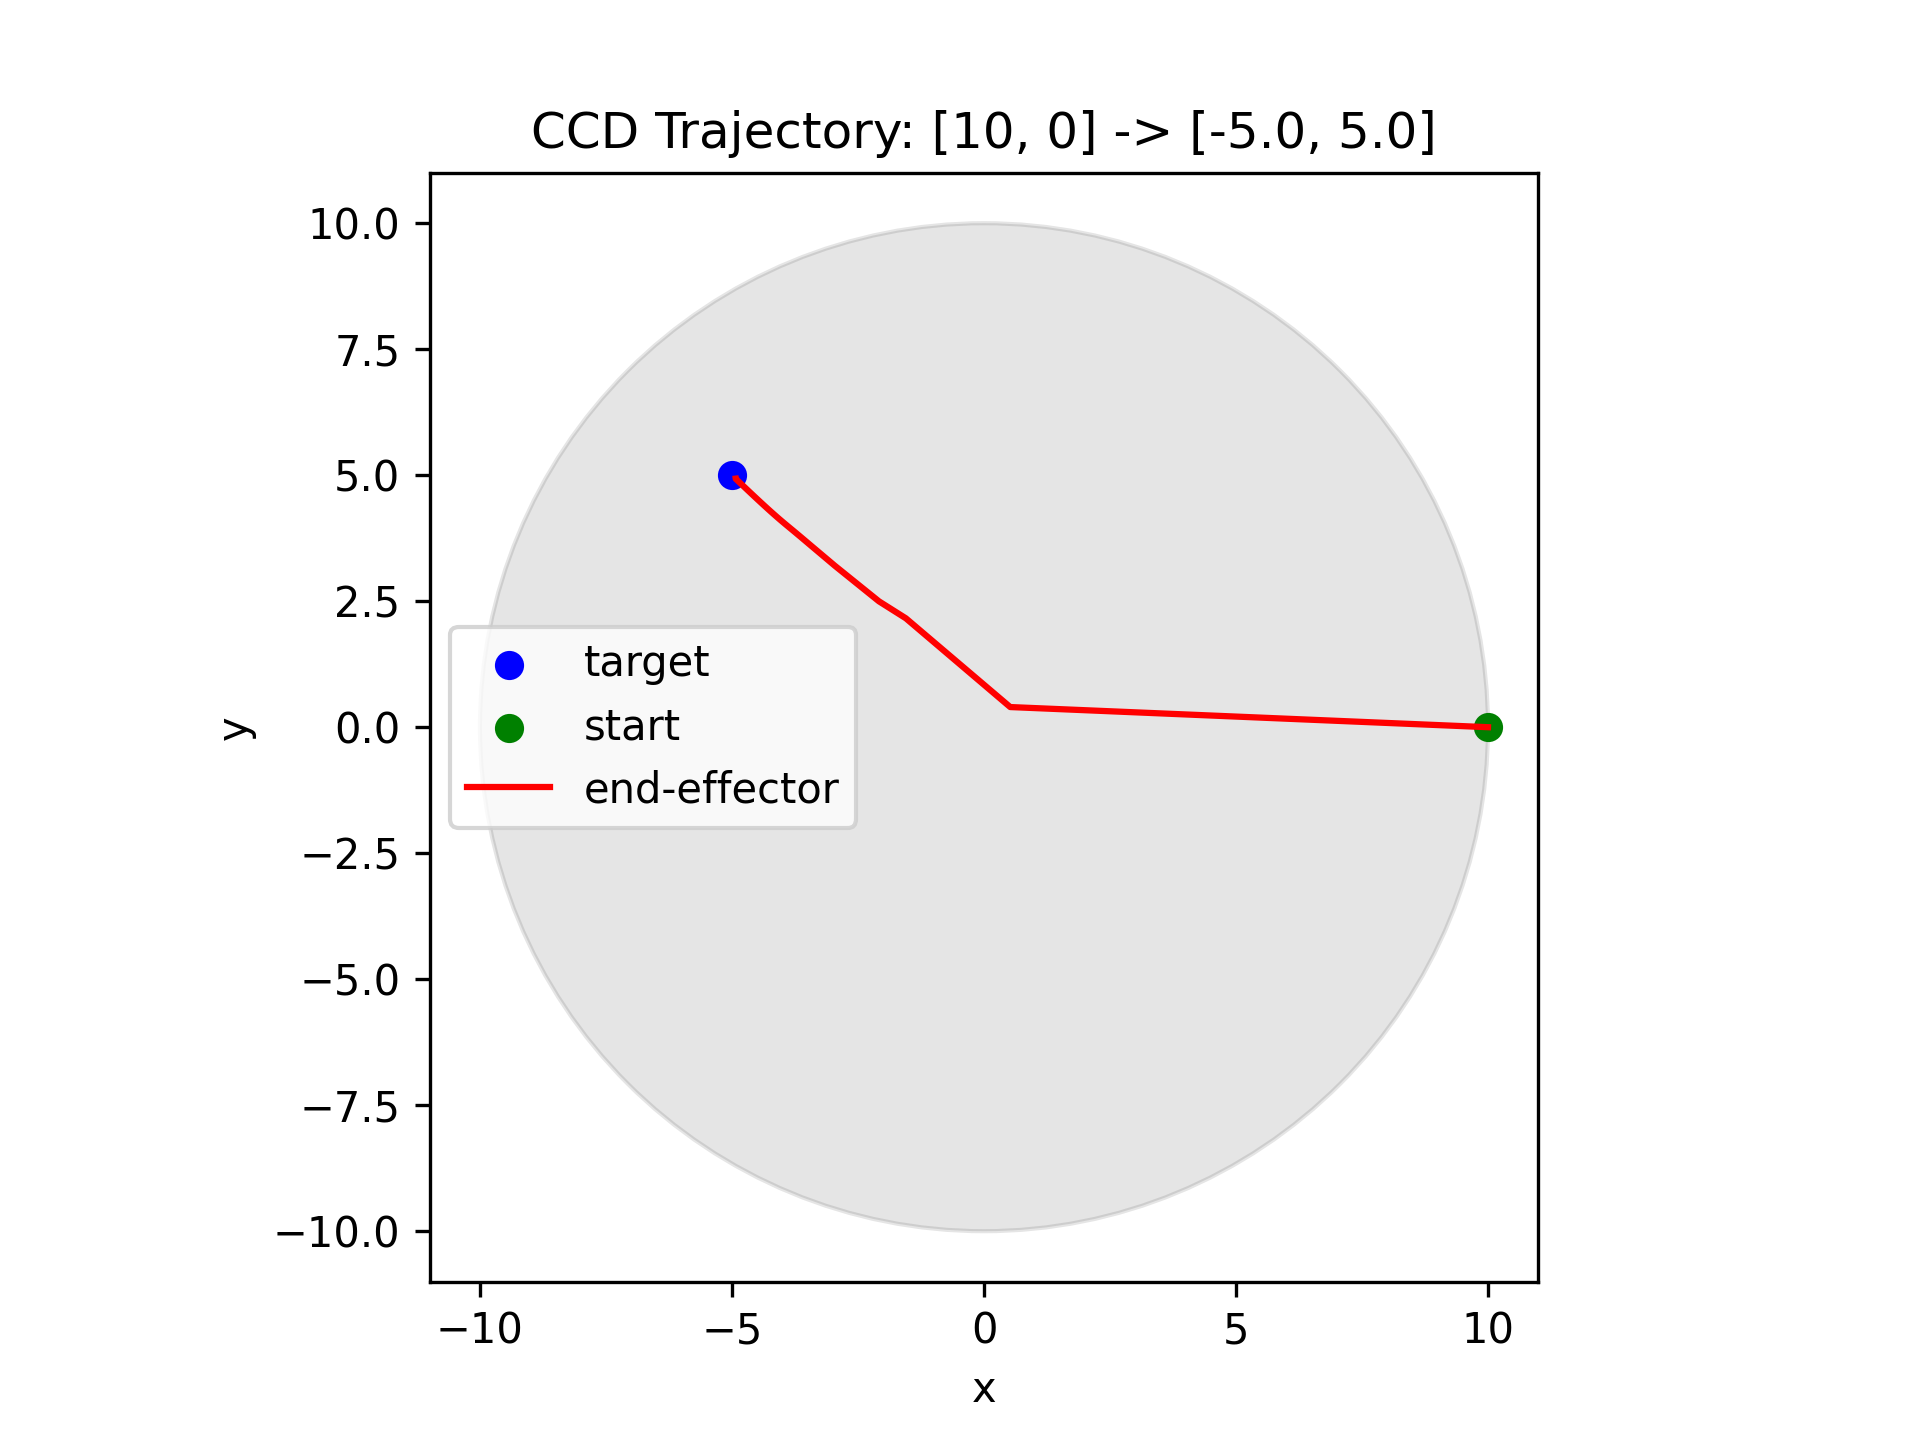
\includegraphics[width=0.31\linewidth]{figures/background/CCD_trajectory_10.png}
            \label{fig:ccd_trajectory/10}
            } 
    \end{center}
    \caption[CCD trajectory]{Trajectory to reach from start position at $[N, 0]$ to target position at $[-\frac{1}{2}N, \frac{1}{2}N]$. The two scattered dots resemble the start end effector position (green) and the target position (blue). The red line is the trajectory of the end effector after each while iterations as in \algoref{alg:CCD}. }
    \label{fig:ccd_trajectory}
\end{figure}

That CCD needs different amounts of while iterations depending on start and end position can be observed in \figref{fig:ccd_iterations}. The heatmap plots the different amounts of while iterations needed to get from a constant start position at $p = [N, 0]$ with all angles equal $0$, to a desired target position. Interesting to see are the patterns emerging in those heatmaps where target positions counter clockwise of the start positions are faster to solve than target positions clockwise to the start positions.
\begin{figure}
    \begin{center}
        \subfloat[$N = 2$]{
            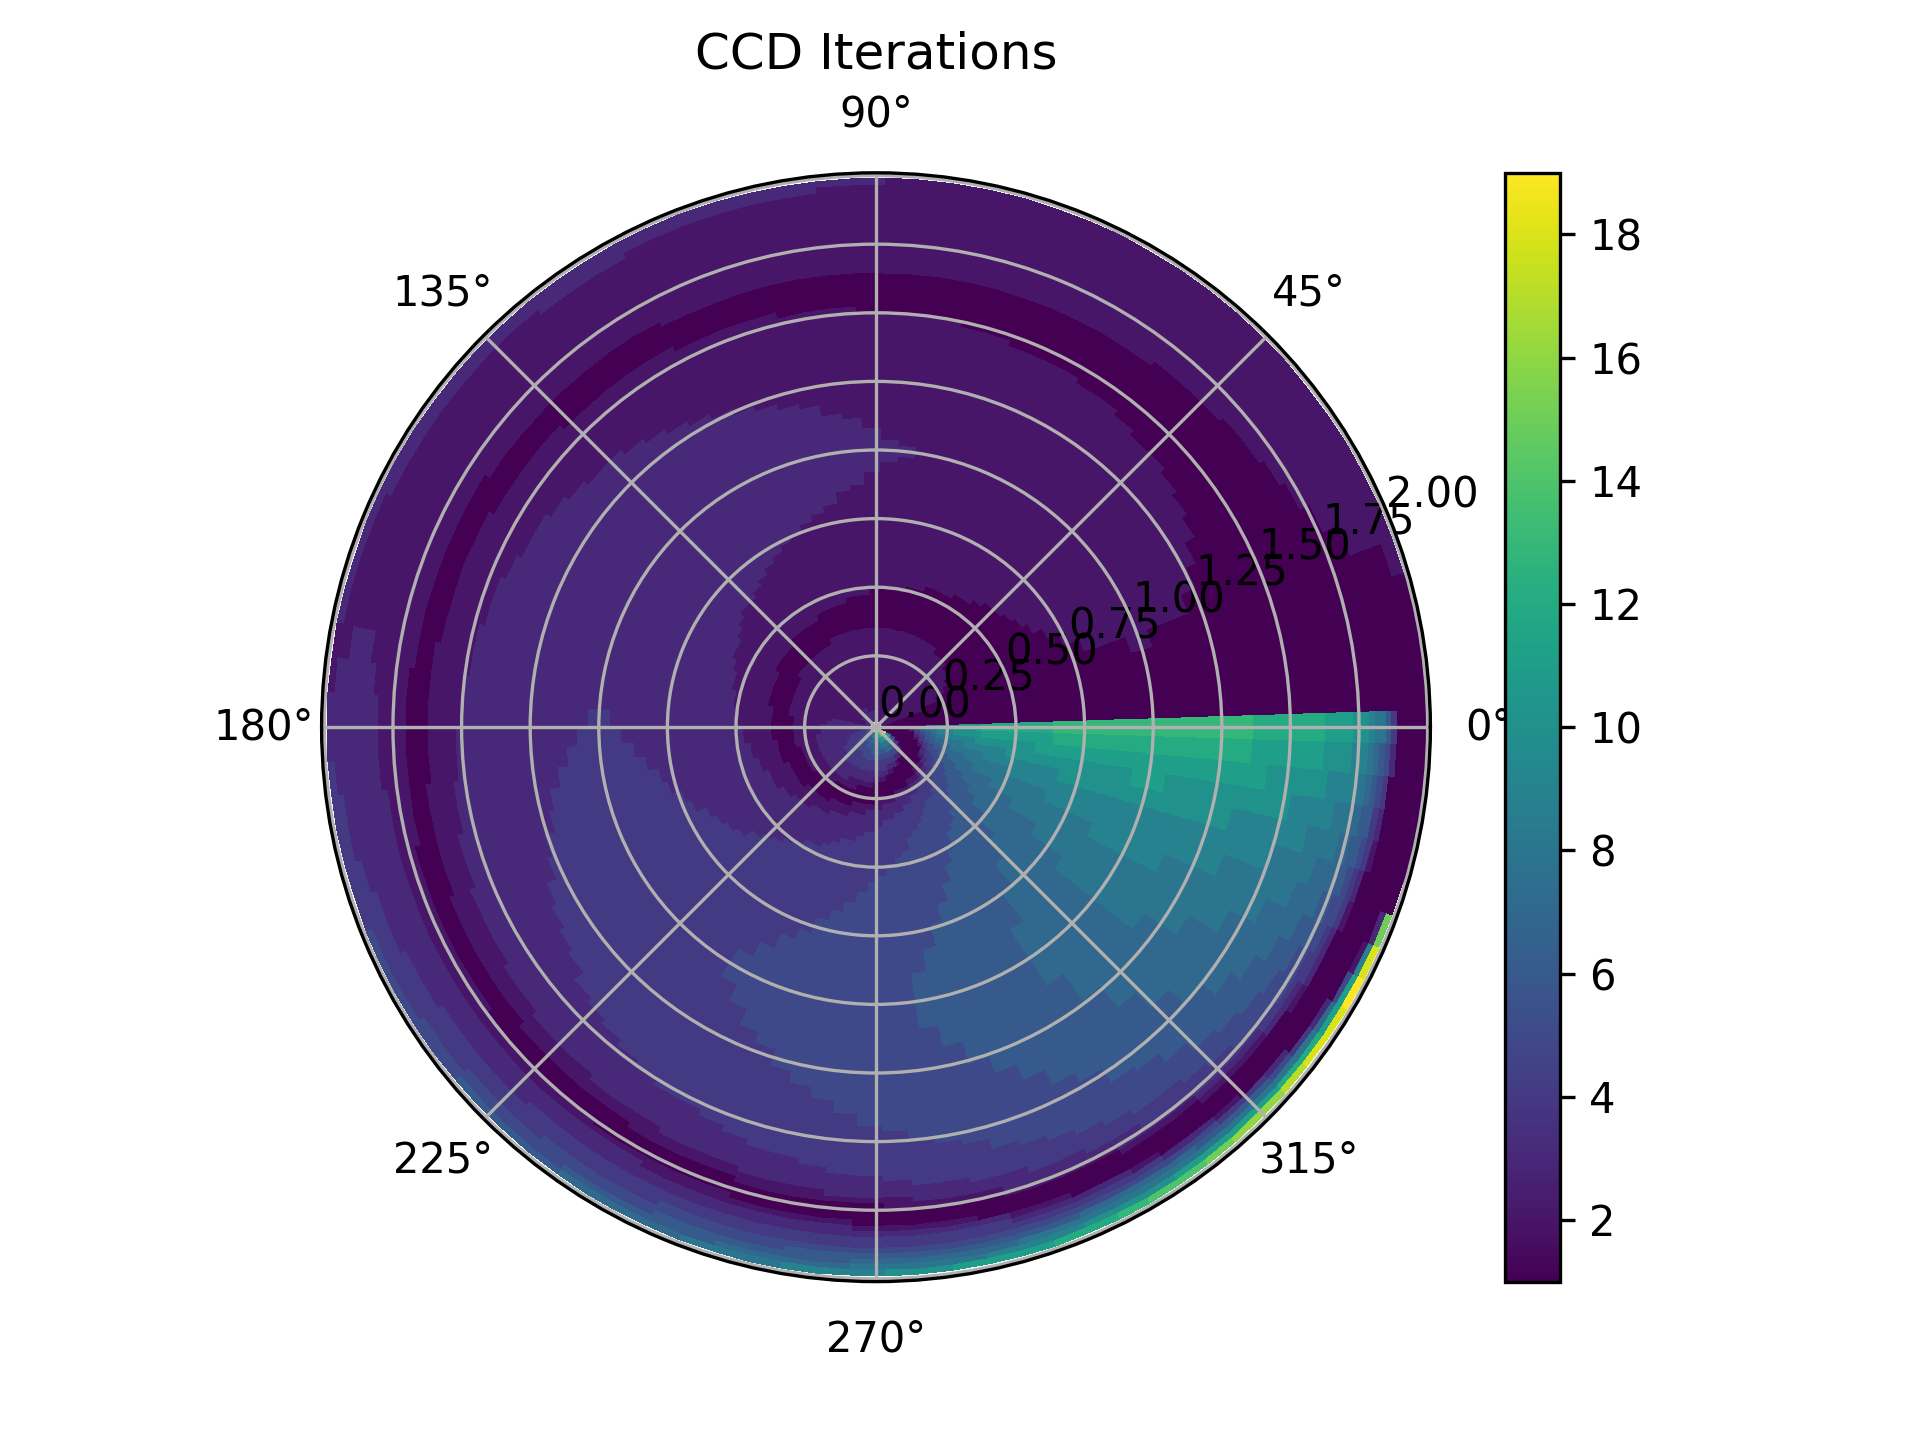
\includegraphics[width=0.31\linewidth]{figures/background/CCD_2_iteration_heatmap.png}
            \label{fig:ccd_iterations/2}
            }
        \hfill
        \subfloat[$N = 5$]{
            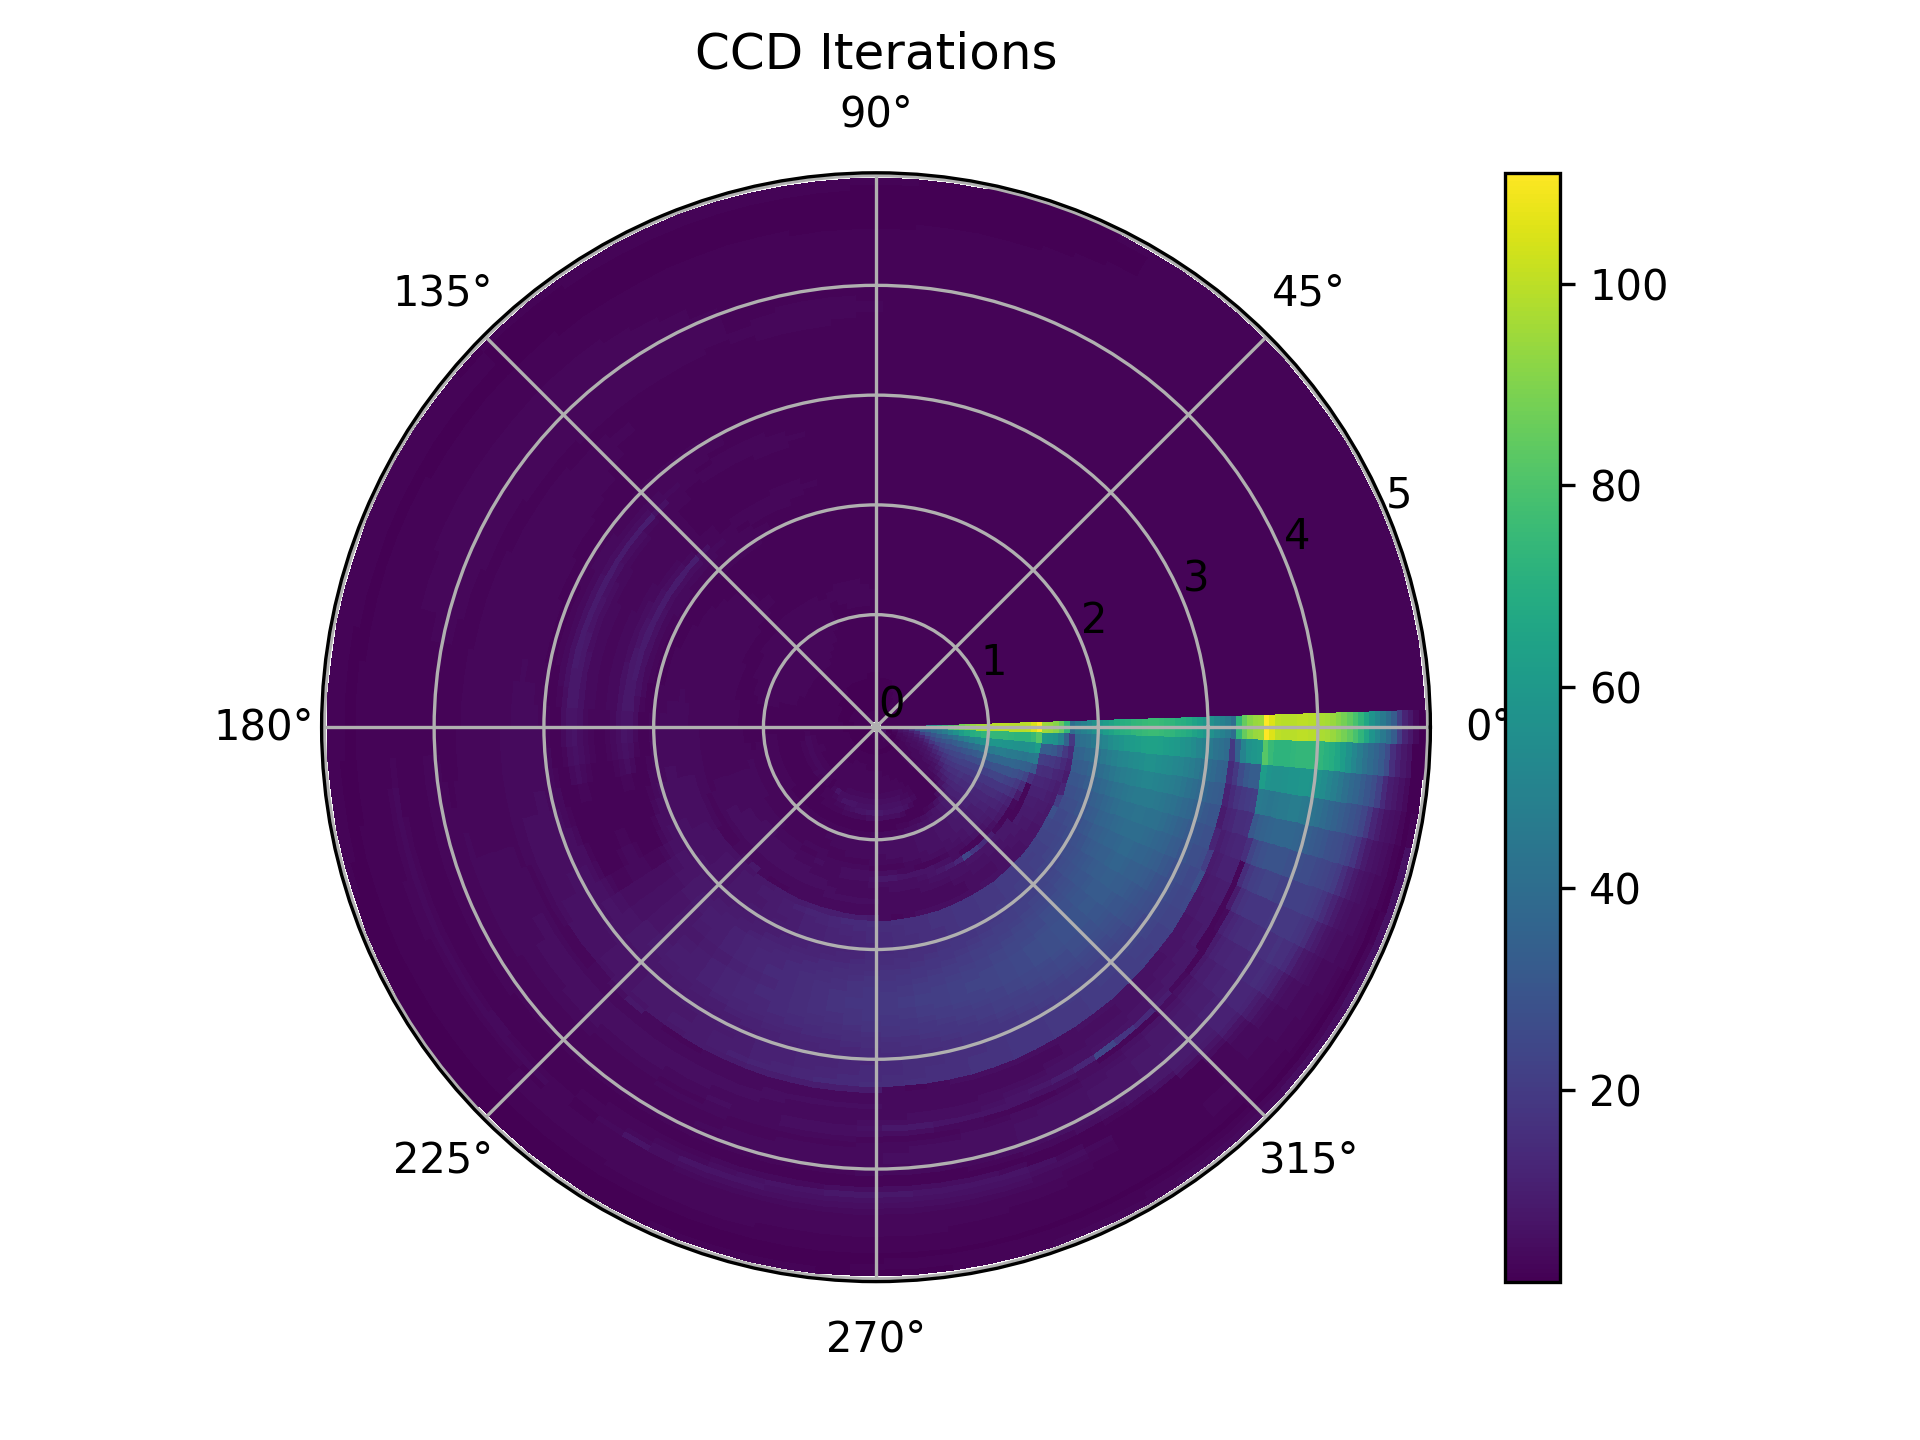
\includegraphics[width=0.31\linewidth]{figures/background/CCD_5_iteration_heatmap.png}
            \label{fig:ccd_iterations/5}
            } 
		\hfill
        \subfloat[$N = 10$]{
            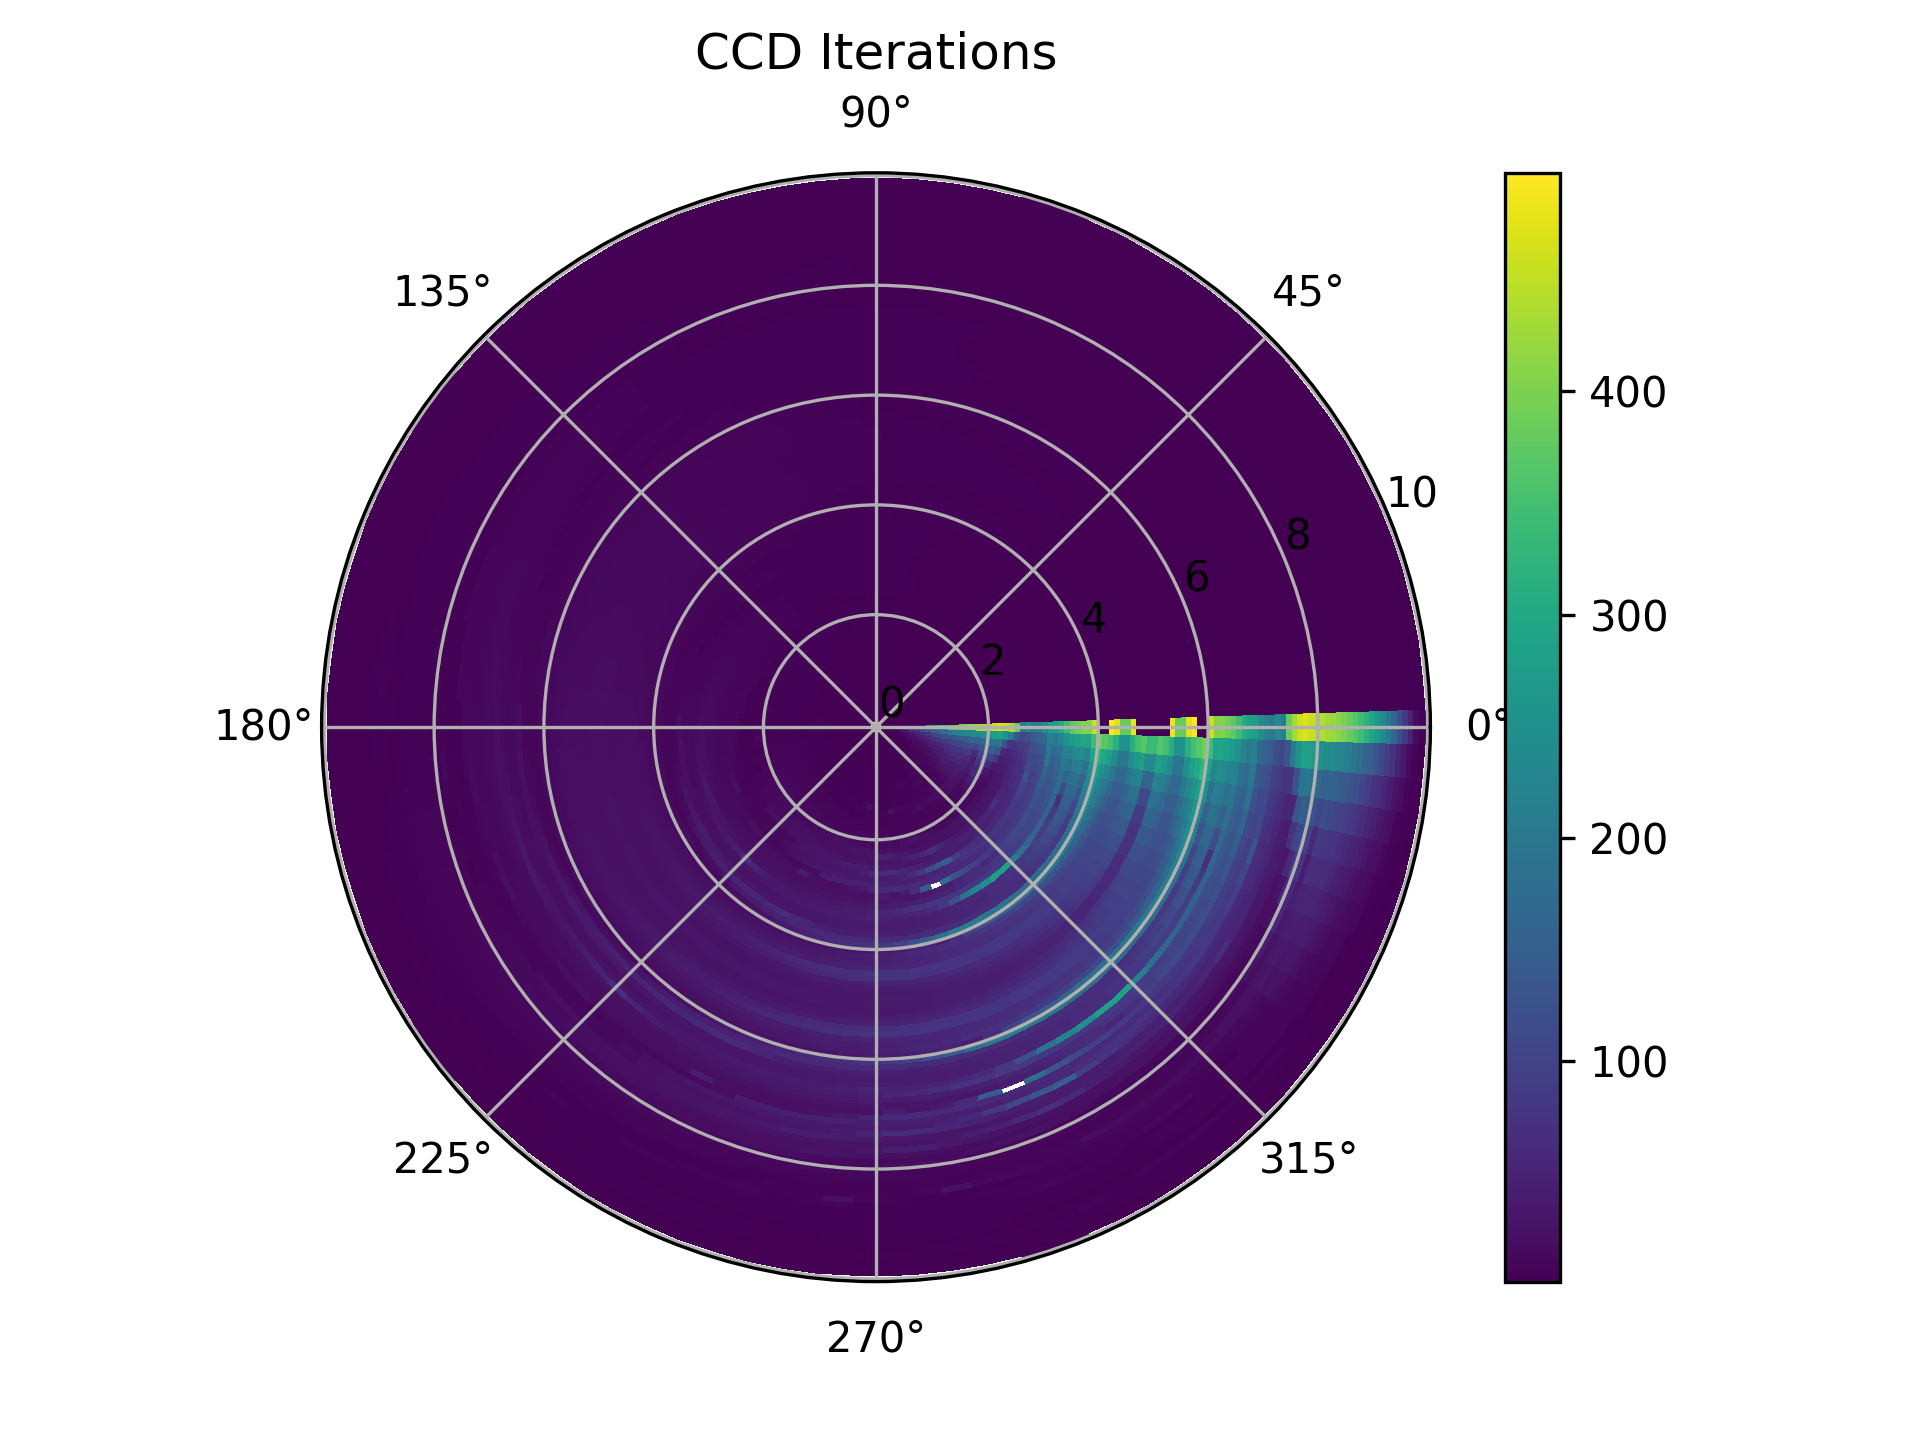
\includegraphics[width=0.31\linewidth]{figures/background/CCD_10_iteration_heatmap.png}
            \label{fig:ccd_iterations/10}
            } 
    \end{center}
    \caption[CCD iteration heatmap]{Heatmaps for iterations needed to reach from a start position at $[N, 0]$ to target positions at $p_{(i, j)} = [\cos(\omega_i), \sin(\omega_i)] \cdot \mathfrak{R}_j, \omega = [0, \ldots, 2\pi), \mathfrak{R}  = [0, \ldots, N]$}
    \label{fig:ccd_iterations}
\end{figure}

